	\newpage
\section{Testowanie}	%5
%Opisujemy testy, sprawdzamy czy nie generuje błędów.


\subsection{Testowanie latarki}

\hspace{0.60cm}Zadania jakie ma spełniać test latarki przedstawione są w tabeli \ref{tab:tablica_latarka}. Jako "X" \\ w kolumnie "Tak" lub "Nie", oznaczamy pomyślny lub niepomyślny przebieg poszczególnych zadań. Całość testu podsumowana jest rzutami ekranu \ref{rys:latarka} wykonanymi podczas testowania jako potwierdzenie wykonanego testu.

\begin{tabela}
	{Testowanie latarki}	%opis w spisie tabel
	{Testowanie latarki}	%opis przy tabeli
	{
		\begin{tabular}{|c|c|c|c|c|} \hline
			\textbf{lp} & \textbf{Zadania do przetestowania} & \textbf{Tak} & \textbf{Nie} \\ \hline
			1 & Latarka po naciśnięciu na guzik włączyła się & X & ~ \\ \hline
			2 & Po włączeniu latarki, guzik zmienia kolor na zielony & X & ~ \\ \hline
			3 & Wyświetlenie komunikatu o włączeniu latarki & X & ~ \\ \hline
			4 & Latarka po naciśnięciu na guzik wyłączyła się & X & ~ \\ \hline
			5 & Po wyłączeniu latarki, guzik zmienia kolor na czerwony & X & ~ \\ \hline
			6 & Wyświetlenie komunikatu o wyłączeniu latarki & X & ~ \\ \hline
		\end{tabular}	}
	\label{tab:tablica_latarka}
\end{tabela}

Rysunek \ref{rys:latarka} przedstawia zrzuty ekranu potwierdzające pomyślny przebieg testu.

\begin{figure}[!hbt]
	\begin{center}
		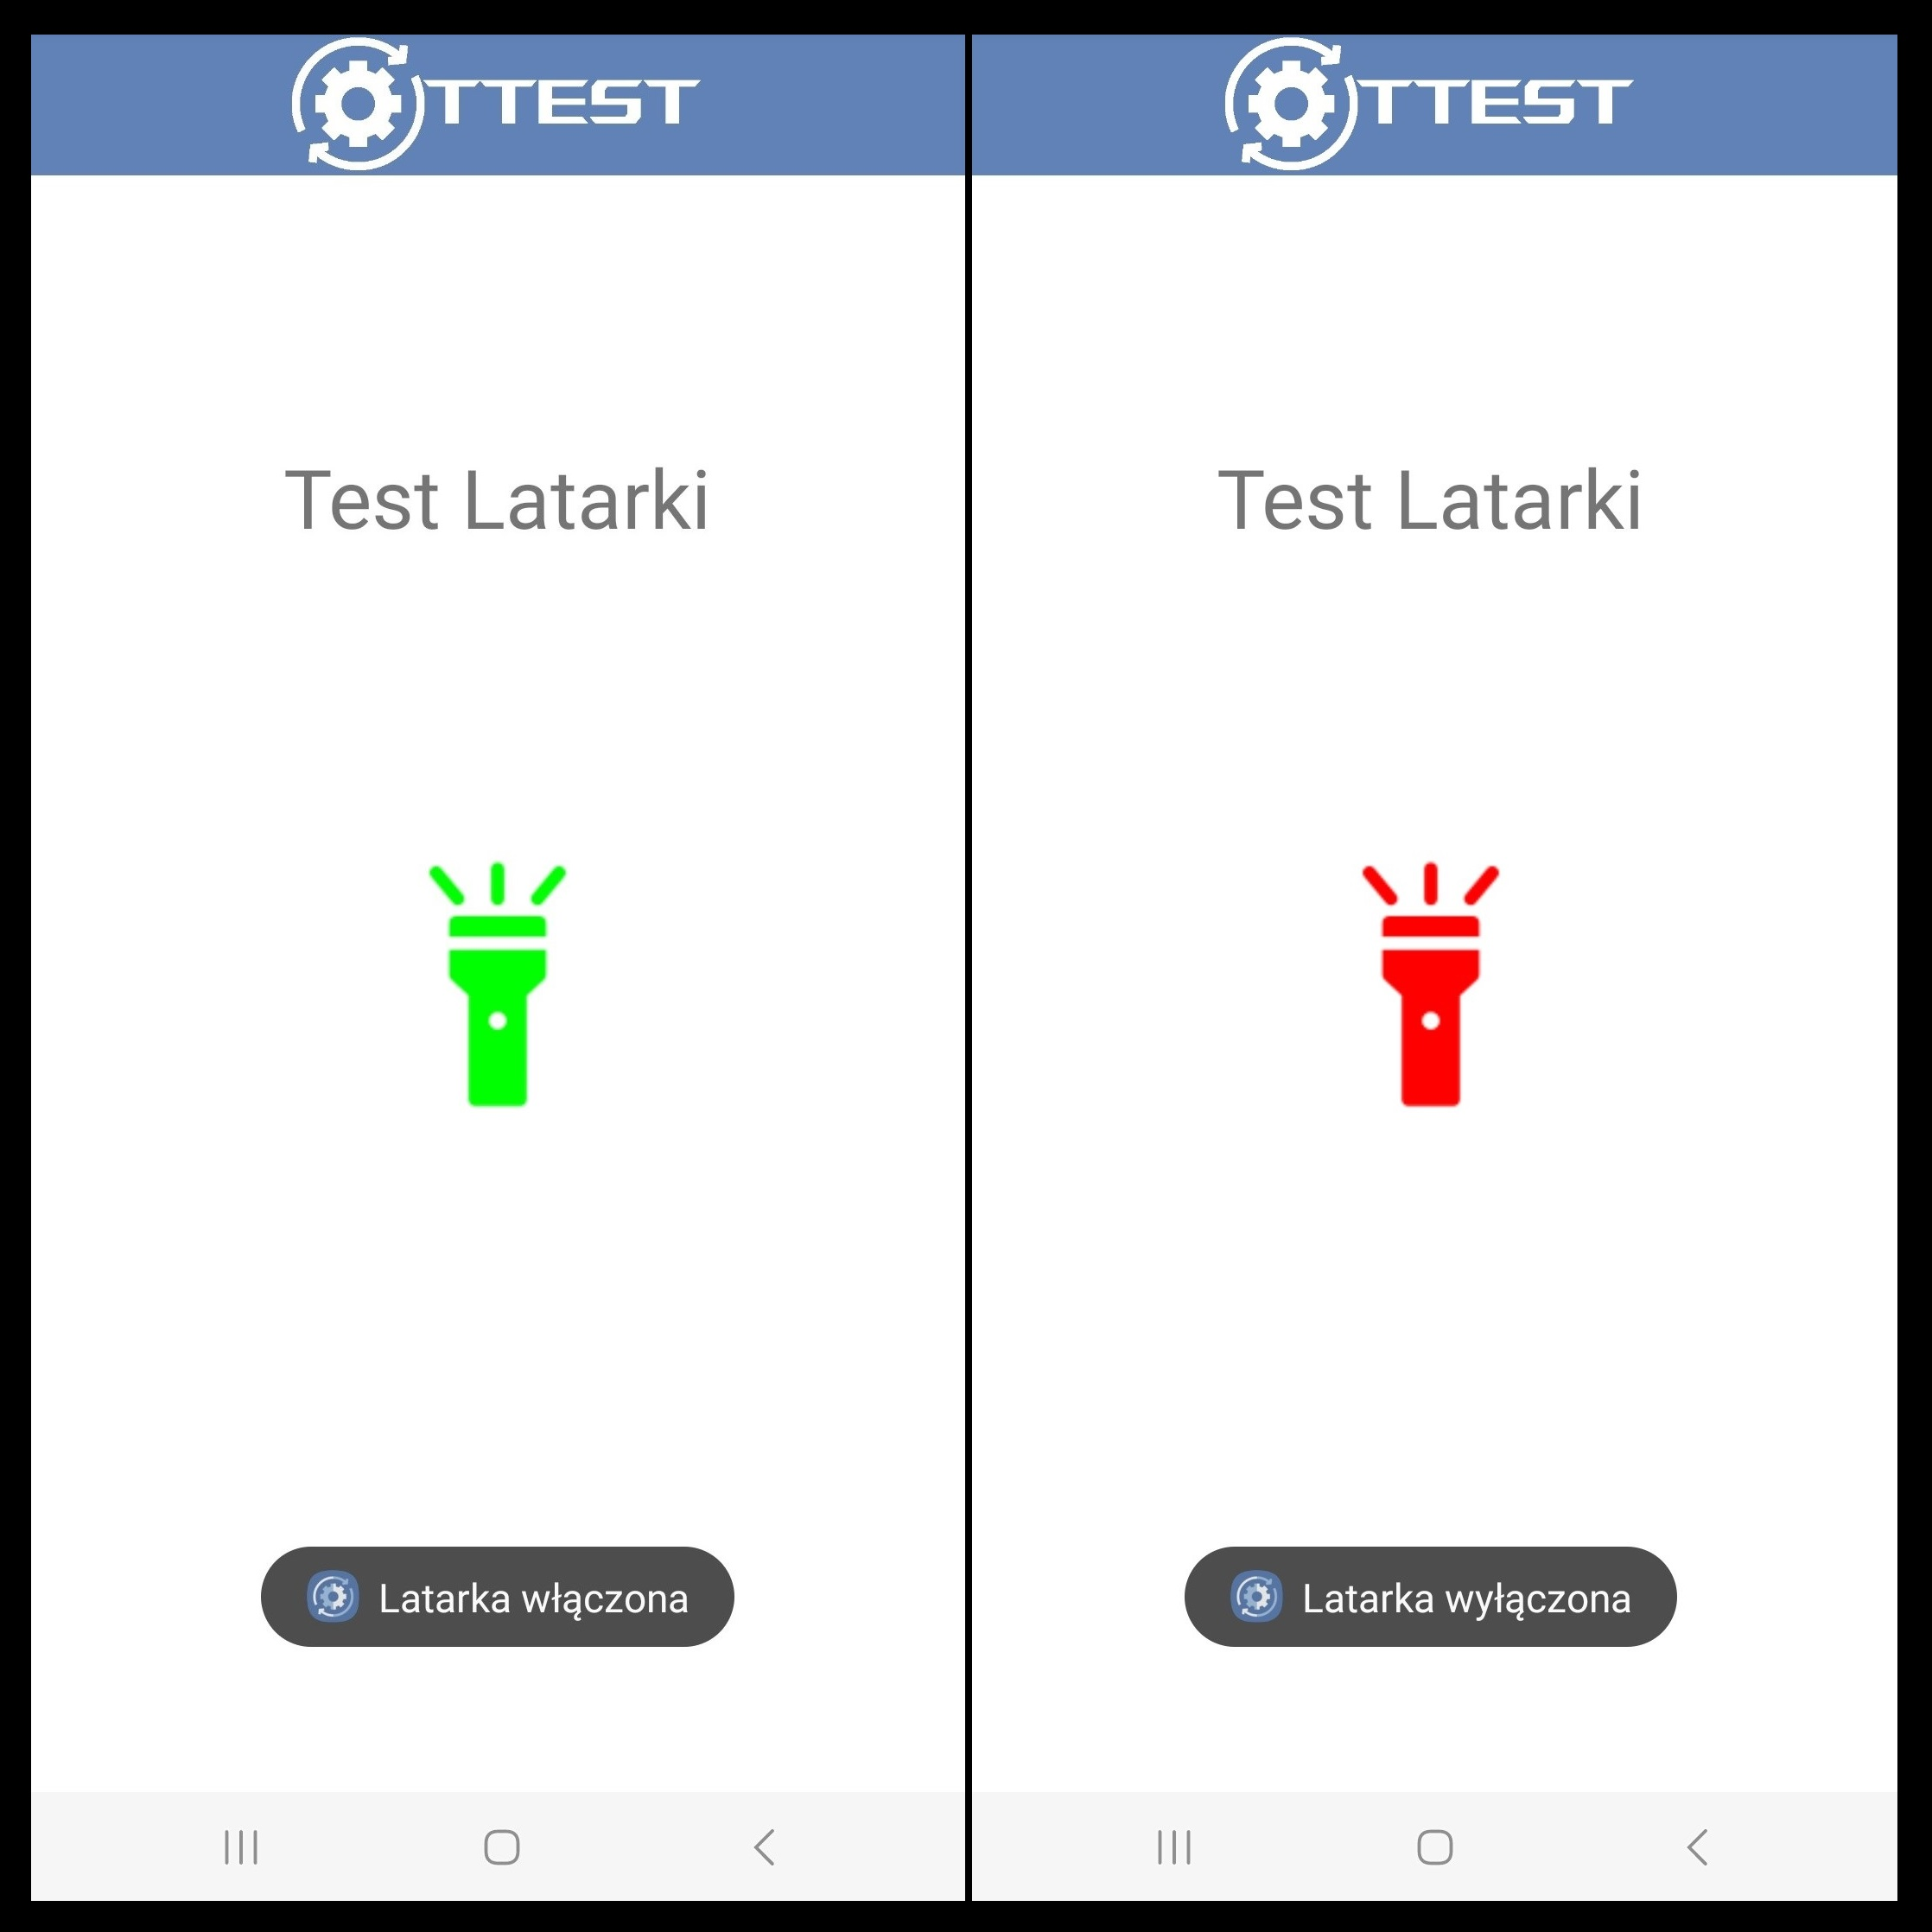
\includegraphics[angle=360, width=0.65\textwidth]{rys/punkt5/latarka.jpg}
		\caption{Przebieg testowania latarki}
		\label{rys:latarka}
	\end{center}
\end{figure}   

\newpage


\subsection{Testowanie trybu ciemnego}

\hspace{0.60cm}Zadania jakie ma spełniać test trybu ciemnego przedstawione są w tabeli \ref{tab:tablica_ciemny}. Jako "X" w kolumnie "Tak" lub "Nie", oznaczamy pomyślny lub niepomyślny przebieg poszczególnych zadań. Całość testu podsumowana jest rzutami ekranu \ref{rys:ciemny} wykonanymi podczas testowania jako potwierdzenie wykonanego testu.

\begin{tabela}
	{Testowanie trybu ciemnego}	%opis w spisie tabel
	{Testowanie trybu ciemnego}	%opis przy tabeli
	{
		\begin{tabular}{|c|c|c|c|c|} \hline
			\textbf{lp} & \textbf{Zadania do przetestowania} & \textbf{Tak} & \textbf{Nie} \\ \hline
			1 & Tryb ciemny po naciśnięciu na guzik włączył się & X & ~ \\ \hline
			2 & Po włączeniu trybu ciemnego, guzik zmienia kolor na zielony & X & ~ \\ \hline
			3 & Wyświetlenie komunikatu o włączeniu trybu ciemnego & X & ~ \\ \hline
			4 & Tryb ciemny po naciśnięciu na guzik wyłączył się & X & ~ \\ \hline
			5 & Po wyłączeniu trybu ciemnego, guzik zmienia kolor na czerwony & X & ~ \\ \hline
			6 & Wyświetlenie komunikatu o wyłączeniu trybu ciemnego & X & ~ \\ \hline
	\end{tabular}	}
	\label{tab:tablica_ciemny}
\end{tabela}

Rysunek \ref{rys:ciemny} przedstawia zrzuty ekranu potwierdzające pomyślny przebieg testu.

\begin{figure}[!hbt]
	\begin{center}
		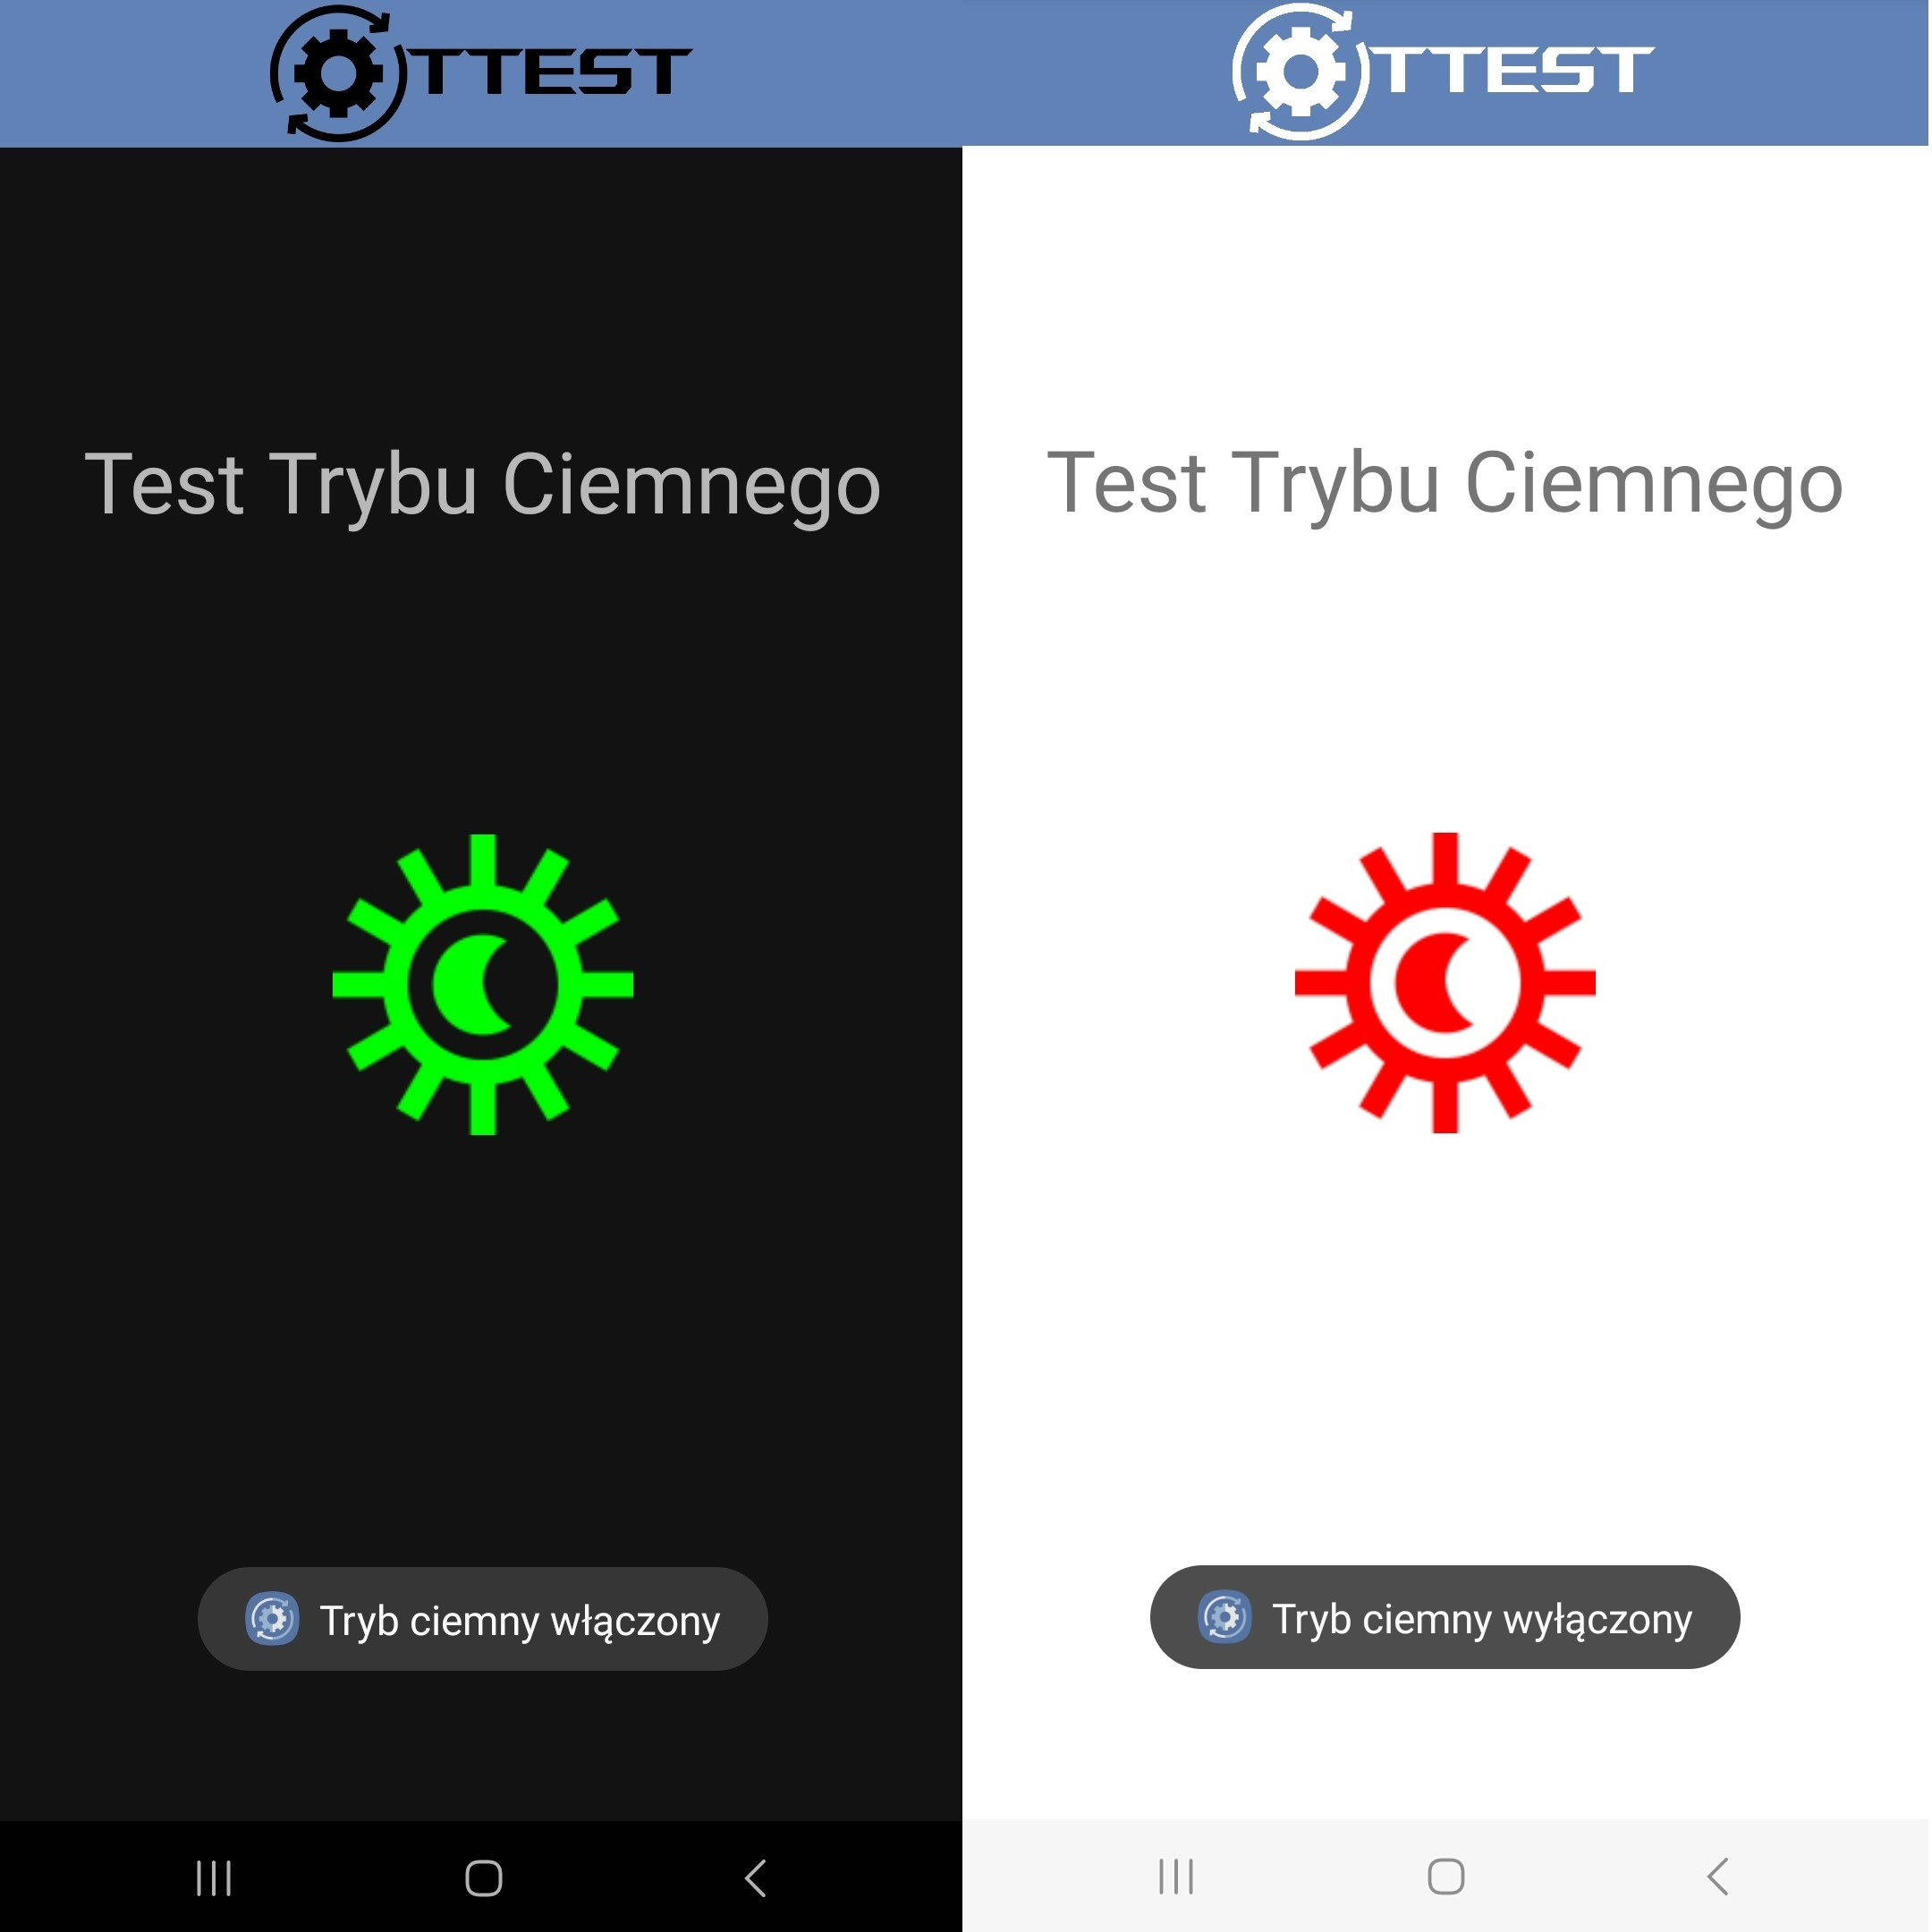
\includegraphics[angle=360, width=0.65\textwidth]{rys/punkt5/ciemny.jpg}
		\caption{Przebieg testowania trybu ciemnego}
		\label{rys:ciemny}
	\end{center}
\end{figure}   

\newpage


\subsection{Testowanie czujnika zbliżeniowego}

\hspace{0.60cm}Zadania jakie ma spełniać test czujnika zbliżeniowego przedstawione są w tabeli \ref{tab:tablica_zblizeniowy}. Jako "X" w kolumnie "Tak" lub "Nie", oznaczamy pomyślny lub niepomyślny przebieg poszczególnych zadań. Całość testu podsumowana jest rzutami ekranu \ref{rys:zblizeniowy} wykonanymi podczas testowania jako potwierdzenie wykonanego testu.

\begin{tabela}
	{Testowanie czujnika zbliżeniowego}	%opis w spisie tabel
	{Testowanie czujnika zbliżeniowego}	%opis przy tabeli
	{
		\begin{tabular}{|c|c|c|c|c|} \hline
			\textbf{lp} & \textbf{Zadania do przetestowania} & \textbf{Tak} & \textbf{Nie} \\ \hline
			1 & Po zbliżeniu obiektu do czujnik zmienia się tekst informacyjny  & X & ~ \\ \hline
			2 & Po oddaleniu obiektu od czujnika zmienia się tekst informacyjny & X & ~ \\ \hline
	\end{tabular}	}
	\label{tab:tablica_zblizeniowy}
\end{tabela}

Rysunek \ref{rys:zblizeniowy} przedstawia zrzuty ekranu potwierdzające pomyślny przebieg testu.

\begin{figure}[!hbt]
	\begin{center}
		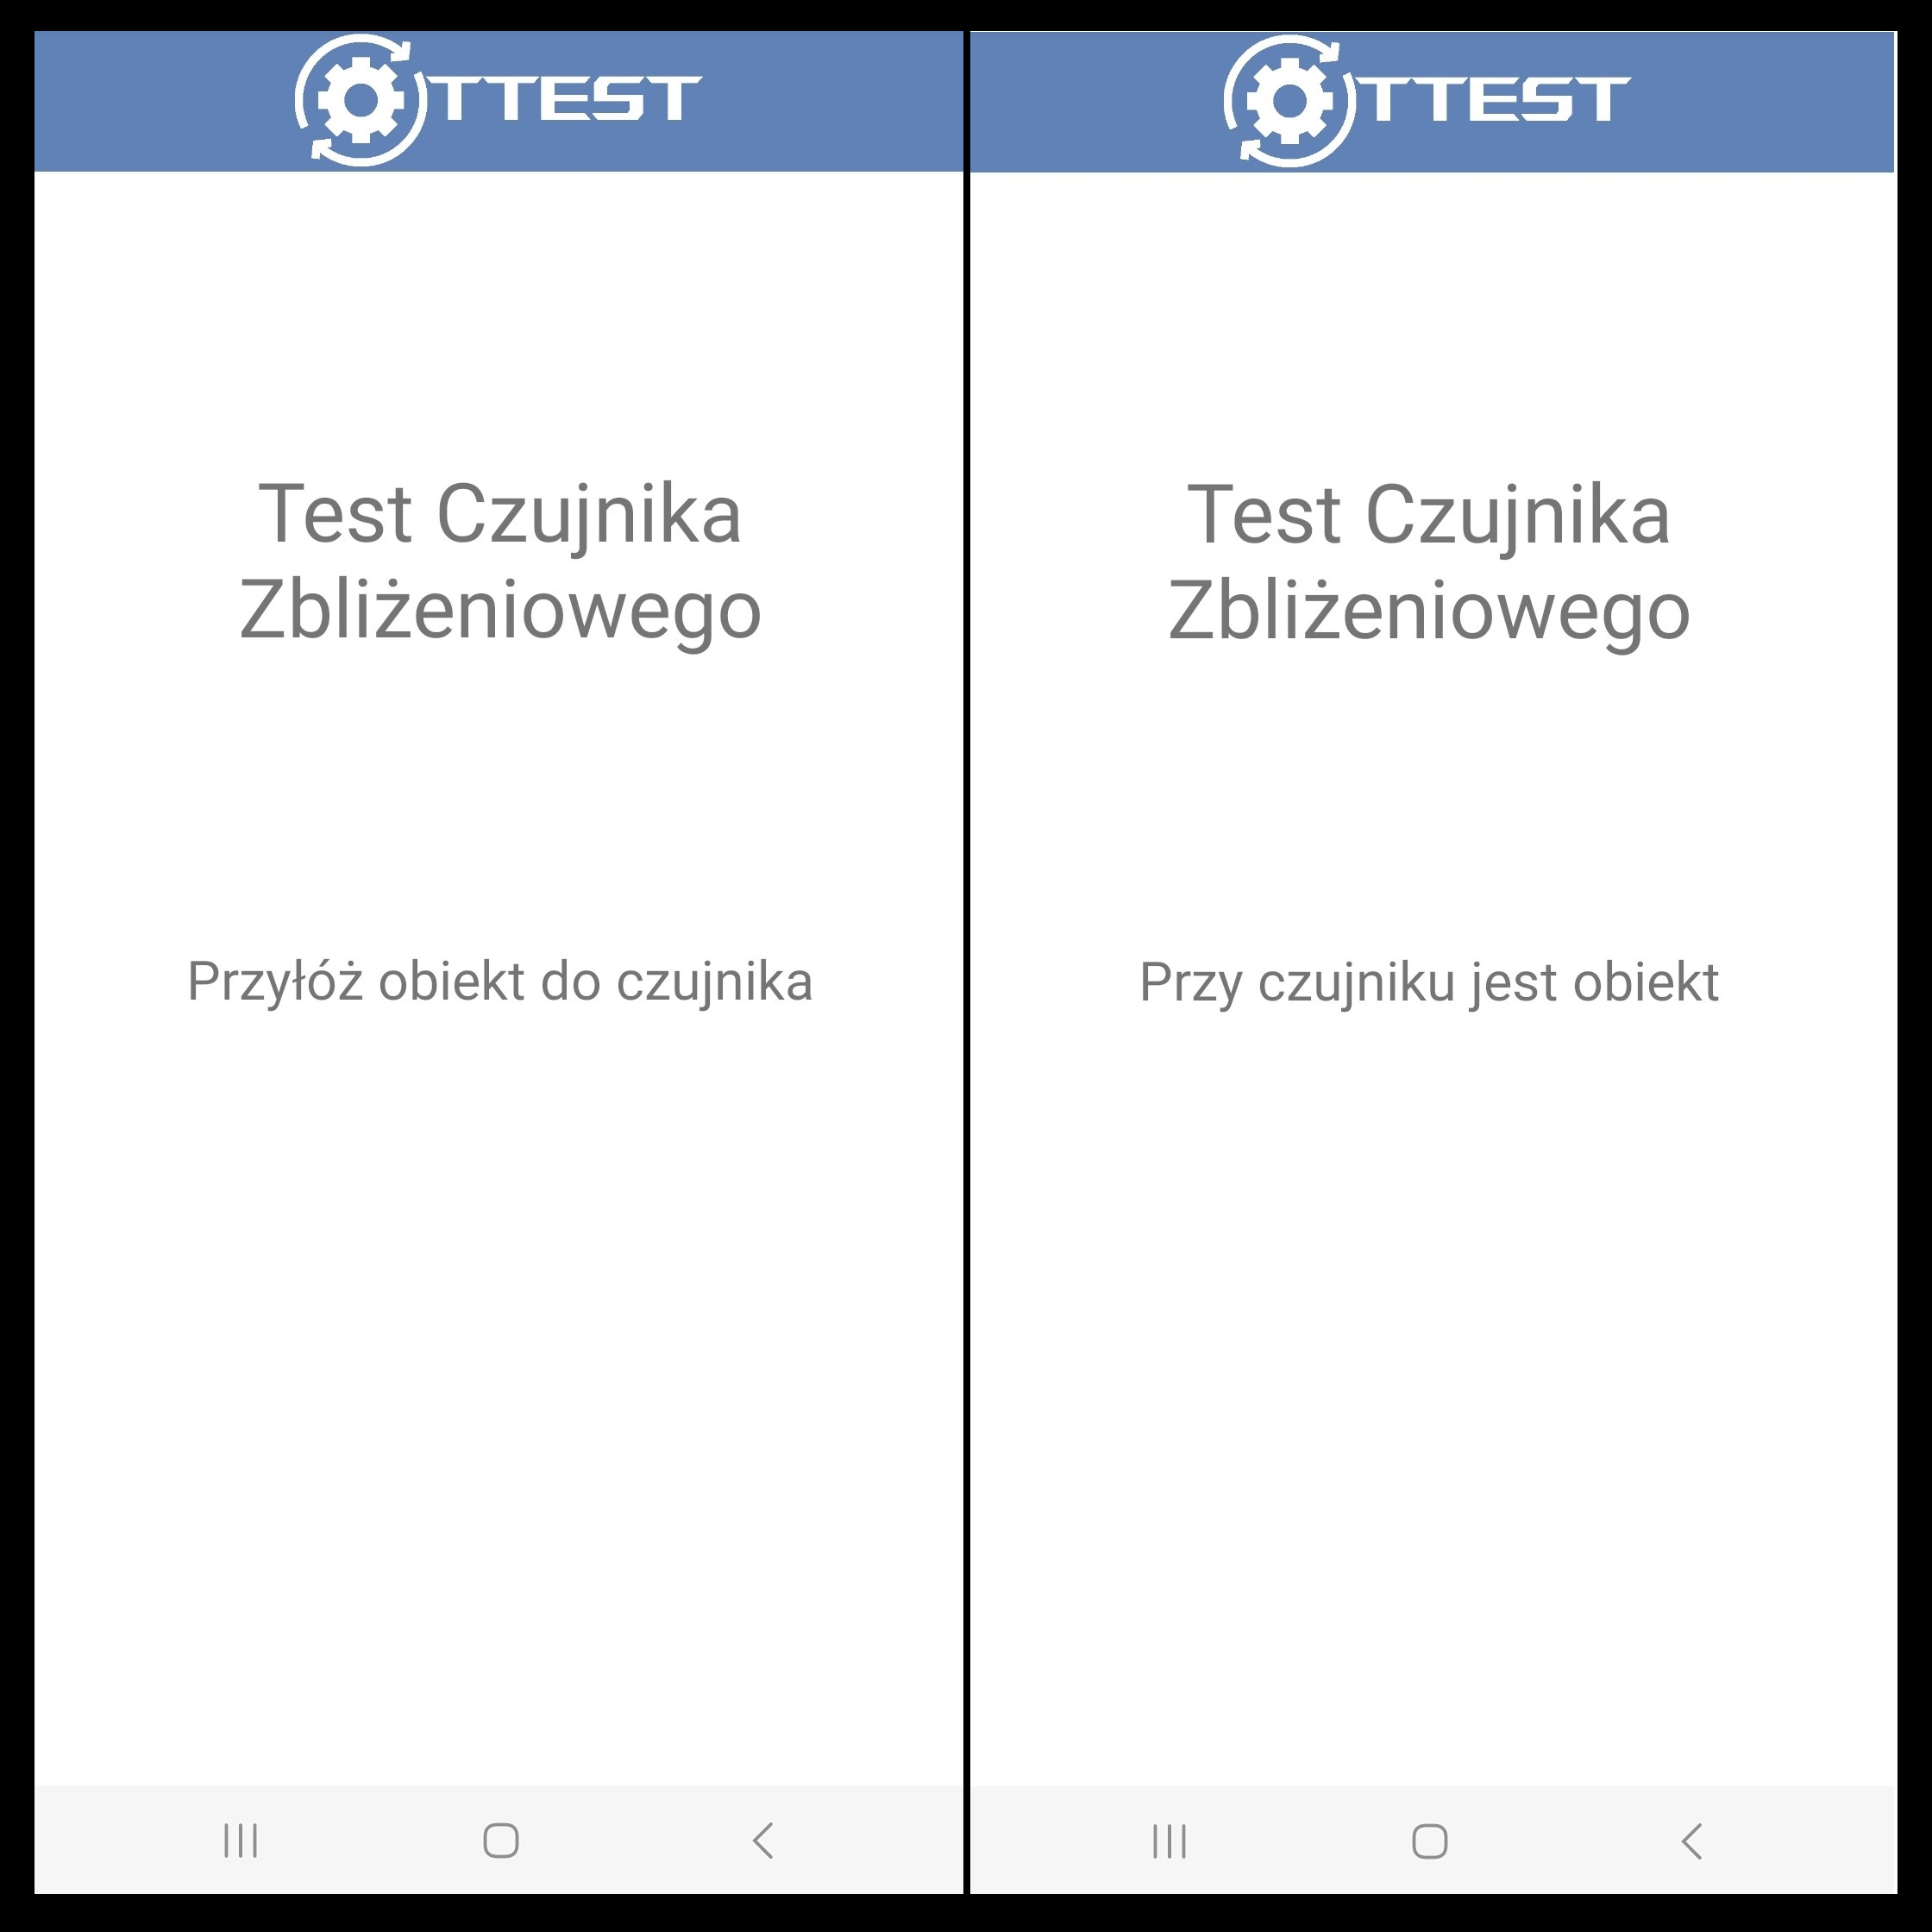
\includegraphics[angle=360, width=0.65\textwidth]{rys/punkt5/zblizeniowy.png}
		\caption{Przebieg testowania czujnika zbliżeniowego}
		\label{rys:zblizeniowy}
	\end{center}
\end{figure}   

\newpage


\subsection{Testowanie lokalizacji}

\hspace{0.60cm}Zadania jakie ma spełniać test lokalizacji przedstawione są w tabeli \ref{tab:tablica_gps}. Jako "X" w kolumnie "Tak" lub "Nie", oznaczamy pomyślny lub niepomyślny przebieg poszczególnych zadań. Całość testu podsumowana jest rzutami ekranu \ref{rys:gps_5} wykonanymi podczas testowania jako potwierdzenie wykonanego testu.

\begin{tabela}
	{Testowanie lokalizacji}	%opis w spisie tabel
	{Testowanie lokalizacji}	%opis przy tabeli
	{
		\begin{tabular}{|c|c|c|c|c|} \hline
			\textbf{lp} & \textbf{Zadania do przetestowania} & \textbf{Tak} & \textbf{Nie} \\ \hline
			1 & Po naciśnięciu na guzik wyświetla się adres obecnej lokalizacji  & X & ~ \\ \hline
			2 & Po naciśnięciu na guzik wyświetla się komunikat z współrzędnymi & X & ~ \\ \hline
	\end{tabular}	}
	\label{tab:tablica_gps}
\end{tabela}

Rysunek \ref{rys:gps_5} przedstawia zrzuty ekranu potwierdzające pomyślny przebieg testu.

\begin{figure}[!hbt]
	\begin{center}
		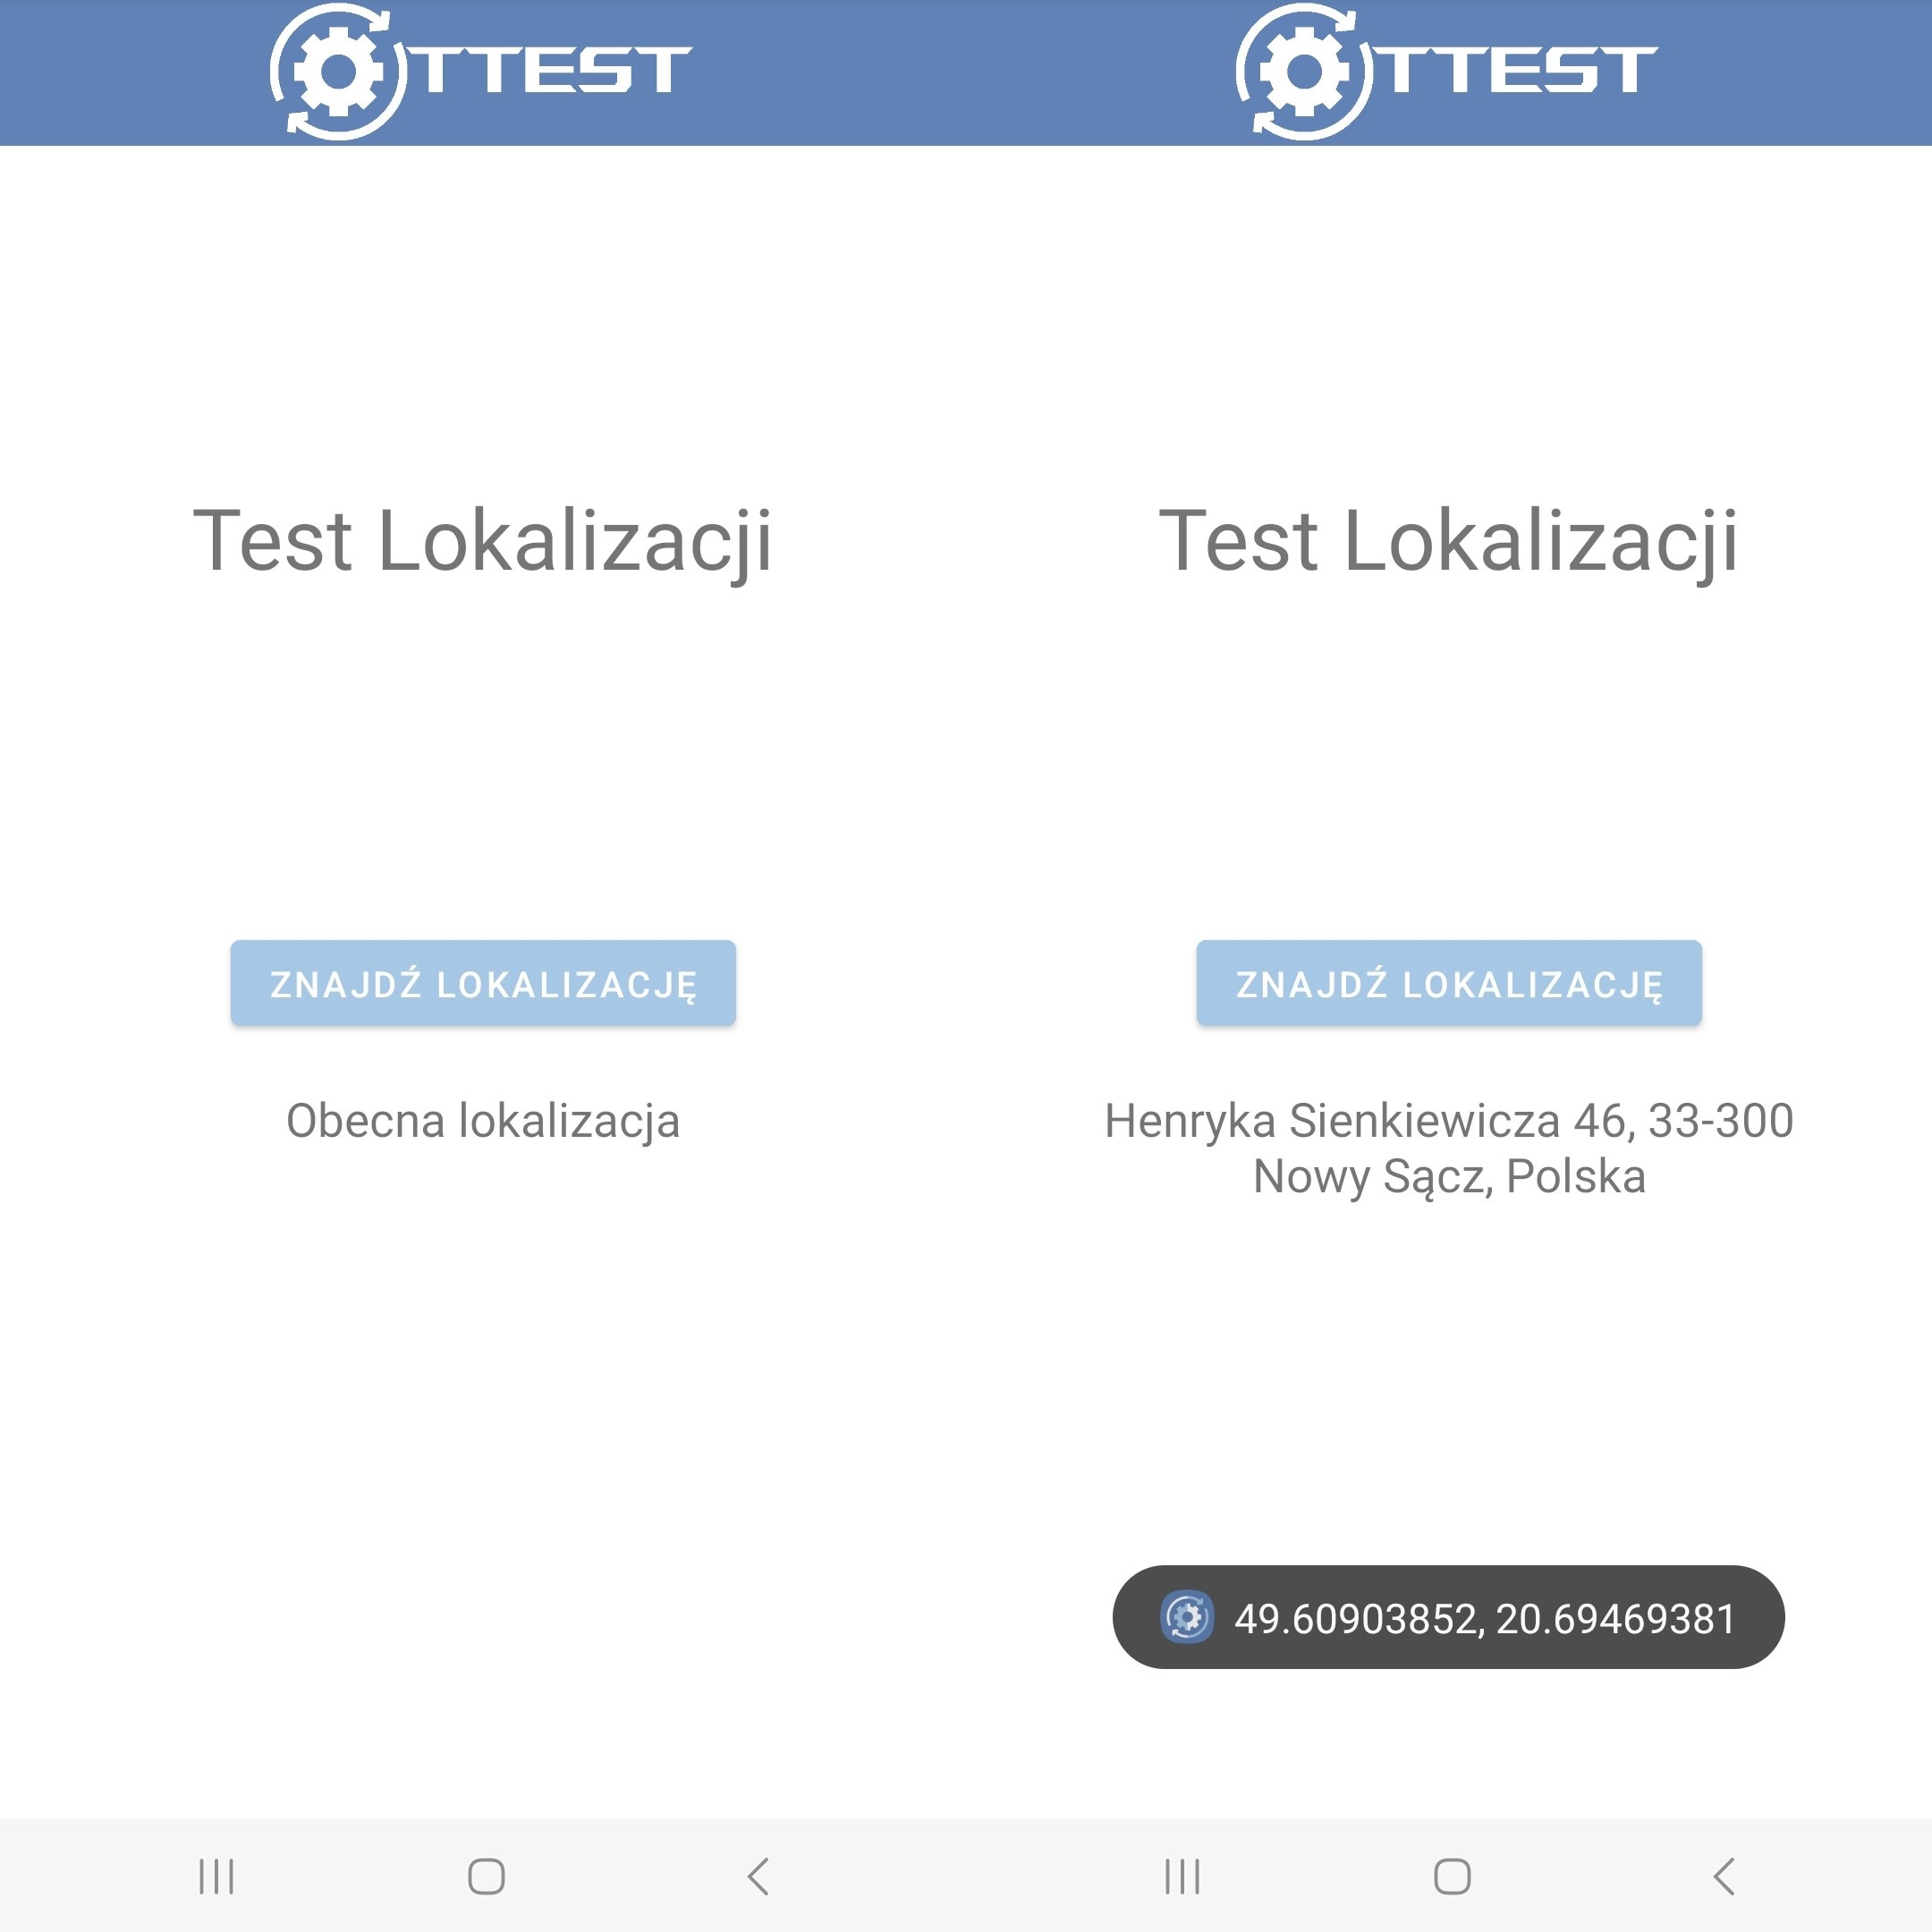
\includegraphics[angle=360, width=0.65\textwidth]{rys/punkt5/gps.jpg}
		\caption{Przebieg testowania lokalizacji}
		\label{rys:gps_5}
	\end{center}
\end{figure} 

\newpage


\subsection{Testowanie wifi}  

\hspace{0.60cm}Zadania jakie ma spełniać test wifi przedstawione są w tabeli \ref{tab:tablica_wifi}. Jako "X" \\ w kolumnie "Tak" lub "Nie", oznaczamy pomyślny lub niepomyślny przebieg poszczególnych zadań. Całość testu podsumowana jest rzutami ekranu \ref{rys:wifi_5} wykonanymi podczas testowania jako potwierdzenie wykonanego testu.

\begin{tabela}
	{Testowanie wifi}	%opis w spisie tabel
	{Testowanie wifi}	%opis przy tabeli
	{
		\begin{tabular}{|c|c|c|c|c|} \hline
			\textbf{lp} & \textbf{Zadania do przetestowania} & \textbf{Tak} & \textbf{Nie} \\ \hline
			1 & Pojawia się informacja o statusie wifi & X & ~ \\ \hline
			2 & Po naciśnięciu na guzik pojawia się adres IP telefonu & X & ~ \\ \hline
			3 & Po naciśnięciu na guzik pojawia się adres MAC routera & X & ~ \\ \hline
			4 & Po naciśnięciu na guzik pojawia się SSID sieci & X & ~ \\ \hline
			5 & Po naciśnięciu na guzik pojawia się wskaźnik mocy & X & ~ \\ \hline
	\end{tabular}	}
	\label{tab:tablica_wifi}
\end{tabela}

Rysunek \ref{rys:wifi_5} przedstawia zrzuty ekranu potwierdzające pomyślny przebieg testu.

\begin{figure}[!hbt]
	\begin{center}
		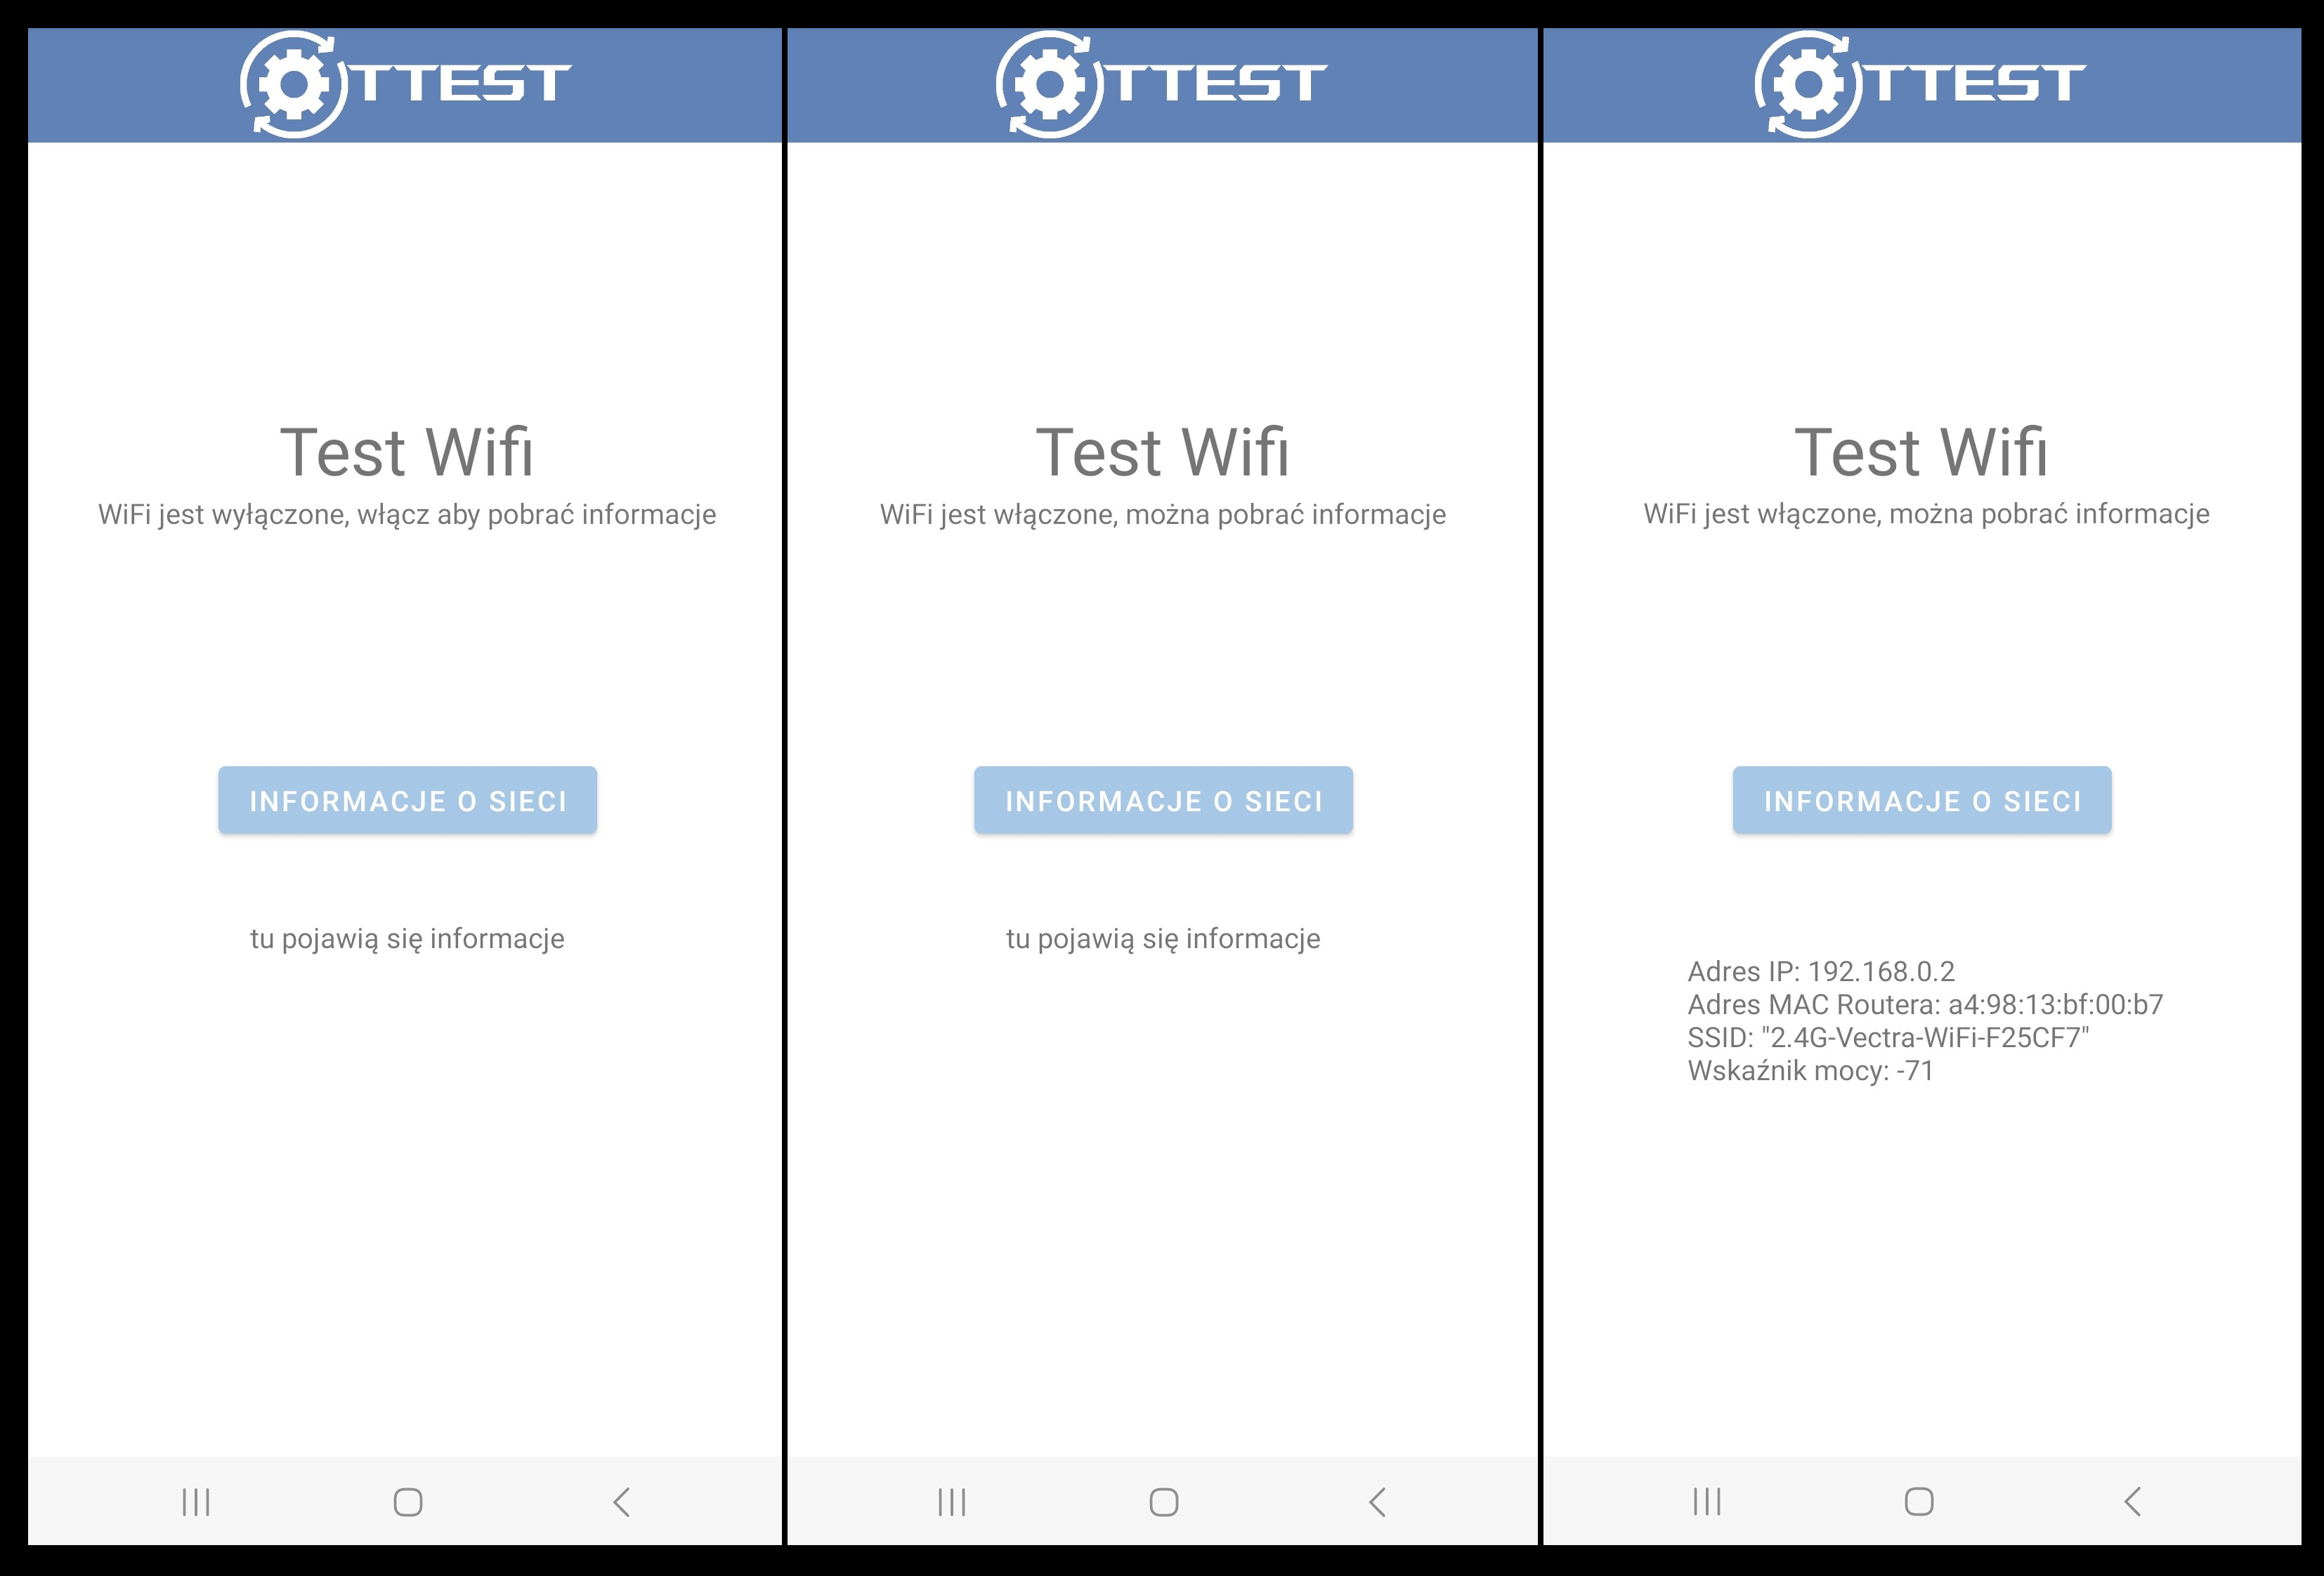
\includegraphics[angle=360, width=0.90\textwidth]{rys/punkt5/wifi.png}
		\caption{Przebieg testowania wifi}
		\label{rys:wifi_5}
	\end{center}
\end{figure} 

\newpage


\subsection{Testowanie dźwięku}

\hspace{0.60cm}Zadania jakie ma spełniać test dźwięku przedstawione są w tabeli \ref{tab:tablica_dzwiek}. Jako "X" \\ w kolumnie "Tak" lub "Nie", oznaczamy pomyślny lub niepomyślny przebieg poszczególnych zadań. Całość testu podsumowana jest rzutami ekranu \ref{rys:dzwiek} wykonanymi podczas testowania jako potwierdzenie wykonanego testu.

\begin{tabela}
	{Testowanie dźwięku}	%opis w spisie tabel
	{Testowanie dźwięku}	%opis przy tabeli
	{
		\begin{tabular}{|c|c|c|c|c|} \hline
			\textbf{lp} & \textbf{Zadania do przetestowania} & \textbf{Tak} & \textbf{Nie} \\ \hline
			1 & Po naciśnięciu na guzik z głośników słychać śpiew ptaków & X & ~ \\ \hline
			2 & Wyświetlenie komunikatu o rozpoczęciu odtwarzania nagrania & X & ~ \\ \hline
	\end{tabular}	}
	\label{tab:tablica_dzwiek}
\end{tabela}

Rysunek \ref{rys:dzwiek} przedstawia zrzuty ekranu potwierdzające pomyślny przebieg testu.

\begin{figure}[!hbt]
	\begin{center}
		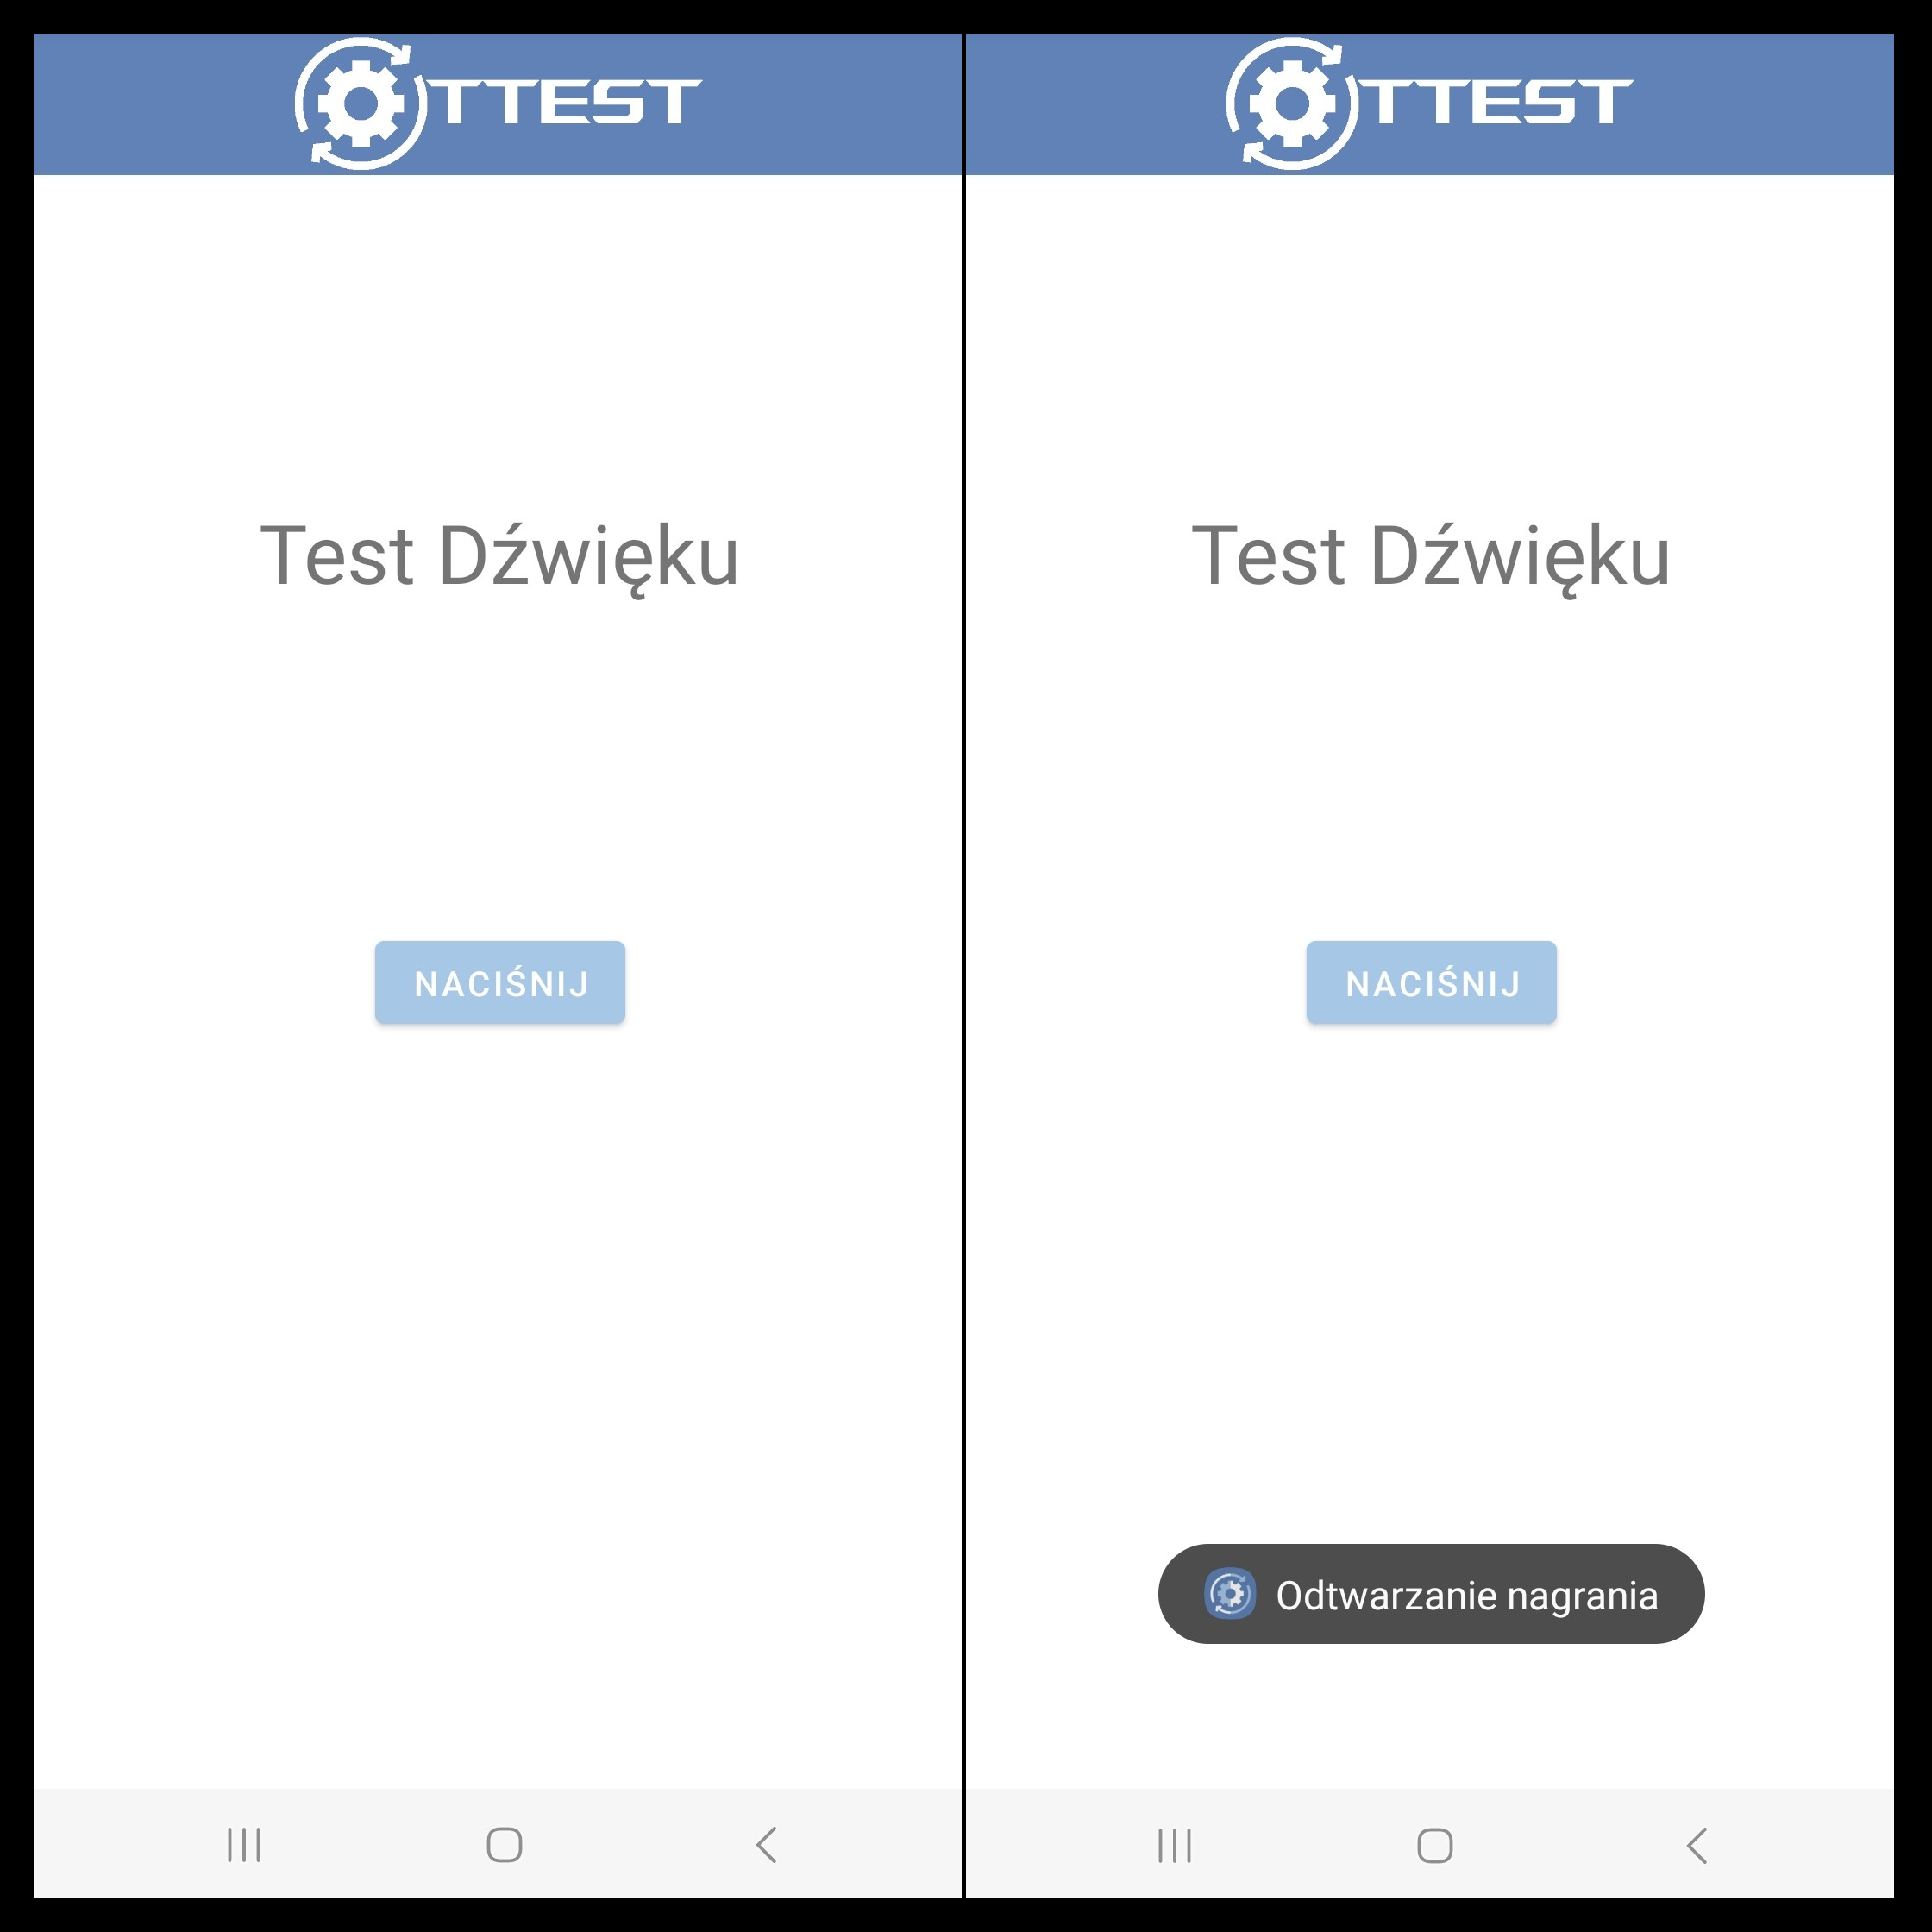
\includegraphics[angle=360, width=0.65\textwidth]{rys/punkt5/dzwiek.png}
		\caption{Przebieg testowania dźwięku}
		\label{rys:dzwiek}
	\end{center}
\end{figure} 

\newpage


\subsection{Testowanie mikrofonu}

\hspace{0.60cm}Zadania jakie ma spełniać test mikrofonu przedstawione są w tabeli \ref{tab:tablica_mikrofon}. Jako "X" w kolumnie "Tak" lub "Nie", oznaczamy pomyślny lub niepomyślny przebieg poszczególnych zadań. Całość testu podsumowana jest rzutami ekranu \ref{rys:mikrofon_5} wykonanymi podczas testowania jako potwierdzenie wykonanego testu.

\begin{tabela}
	{Testowanie mikrofonu}	%opis w spisie tabel
	{Testowanie mikrofonu}	%opis przy tabeli
	{
		\begin{tabular}{|c|c|c|c|c|} \hline
			\textbf{lp} & \textbf{Zadania do przetestowania} & \textbf{Tak} & \textbf{Nie} \\ \hline
			1 & Naciśnięcie na guzik "START" zaczyna nagrywanie & X & ~ \\ \hline
			2 & Po naciśnięciu na guzik "START" wyświetla się adekwatny komunikat & X & ~ \\ \hline
			3 & Naciśnięcie na guzik "STOP" kończy nagrywanie & X & ~ \\ \hline
			4 & Po naciśnięciu na guzik "STOP" wyświetla się adekwatny komunikat & X & ~ \\ \hline
			5 & Naciśnięcie na guzik "PLAY" odtwarza nagranie & X & ~ \\ \hline
			6 &  Po naciśnięciu na guzik "PLAY" wyświetla się adekwatny komunikat & X & ~ \\ \hline
	\end{tabular}	}
	\label{tab:tablica_mikrofon}
\end{tabela}

Rysunek \ref{rys:mikrofon_5} przedstawia zrzuty ekranu potwierdzające pomyślny przebieg testu.

\begin{figure}[!hbt]
	\begin{center}
		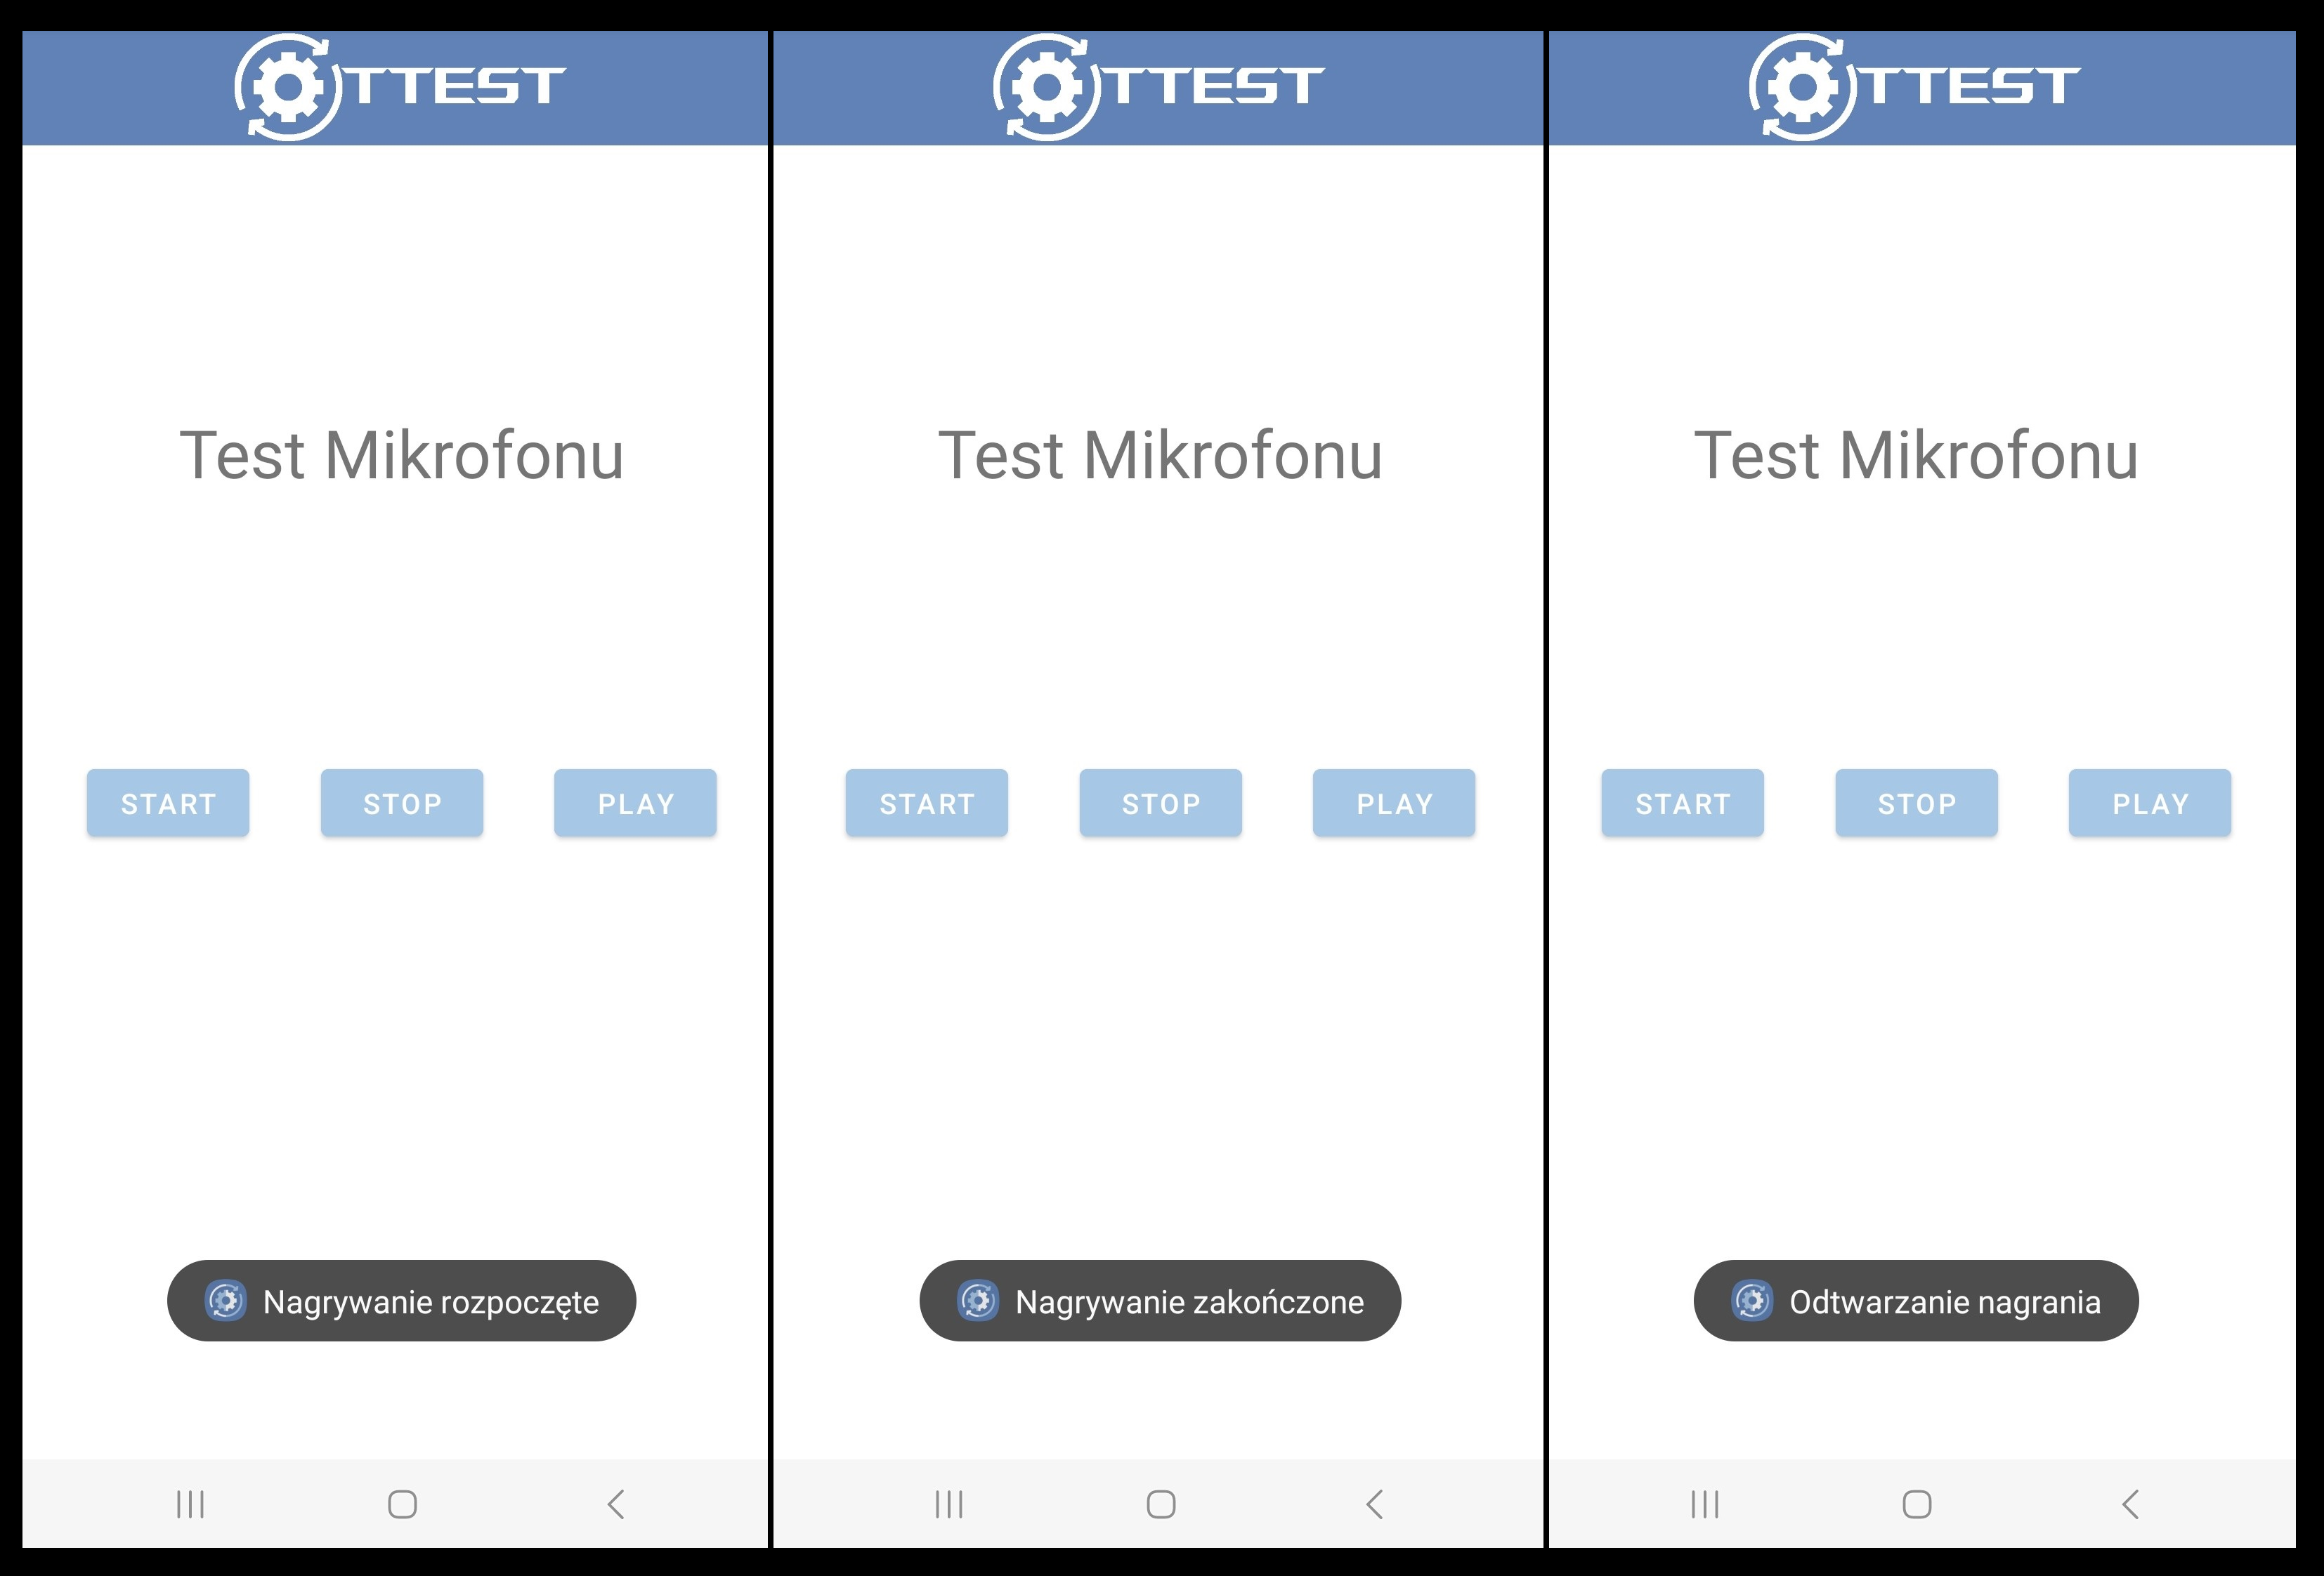
\includegraphics[angle=360, width=0.90\textwidth]{rys/punkt5/mikrofon.png}
		\caption{Przebieg testowania mikrofonu}
		\label{rys:mikrofon_5}
	\end{center}
\end{figure} 

\newpage


\subsection{Testowanie aparatu}

\hspace{0.60cm}Zadania jakie ma spełniać test mikrofonu przedstawione są w tabeli \ref{tab:tablica_aparat}. Jako "X" w kolumnie "Tak" lub "Nie", oznaczamy pomyślny lub niepomyślny przebieg poszczególnych zadań. Całość testu podsumowana jest rzutami ekranu \ref{rys:aparat_5} wykonanymi podczas testowania jako potwierdzenie wykonanego testu.

\begin{tabela}
	{Testowanie aparatu}	%opis w spisie tabel
	{Testowanie aparatu}	%opis przy tabeli
	{
		\begin{tabular}{|c|c|c|c|c|} \hline
			\textbf{lp} & \textbf{Zadania do przetestowania} & \textbf{Tak} & \textbf{Nie} \\ \hline
			1 & Po naciśnięciu na guzik włącza się aplikacja aparatu & X & ~ \\ \hline
			2 & Można wykonać zdjęcie poprzez naciśnięcie białego guzika & X & ~ \\ \hline
			3 & Jako potwierdzenie wykonania zdjęcia, wyświetla się ono & X & ~ \\ \hline
	\end{tabular}	}
	\label{tab:tablica_aparat}
\end{tabela}

Rysunek \ref{rys:aparat_5} przedstawia zrzuty ekranu potwierdzające pomyślny przebieg testu.

\begin{figure}[!hbt]
	\begin{center}
		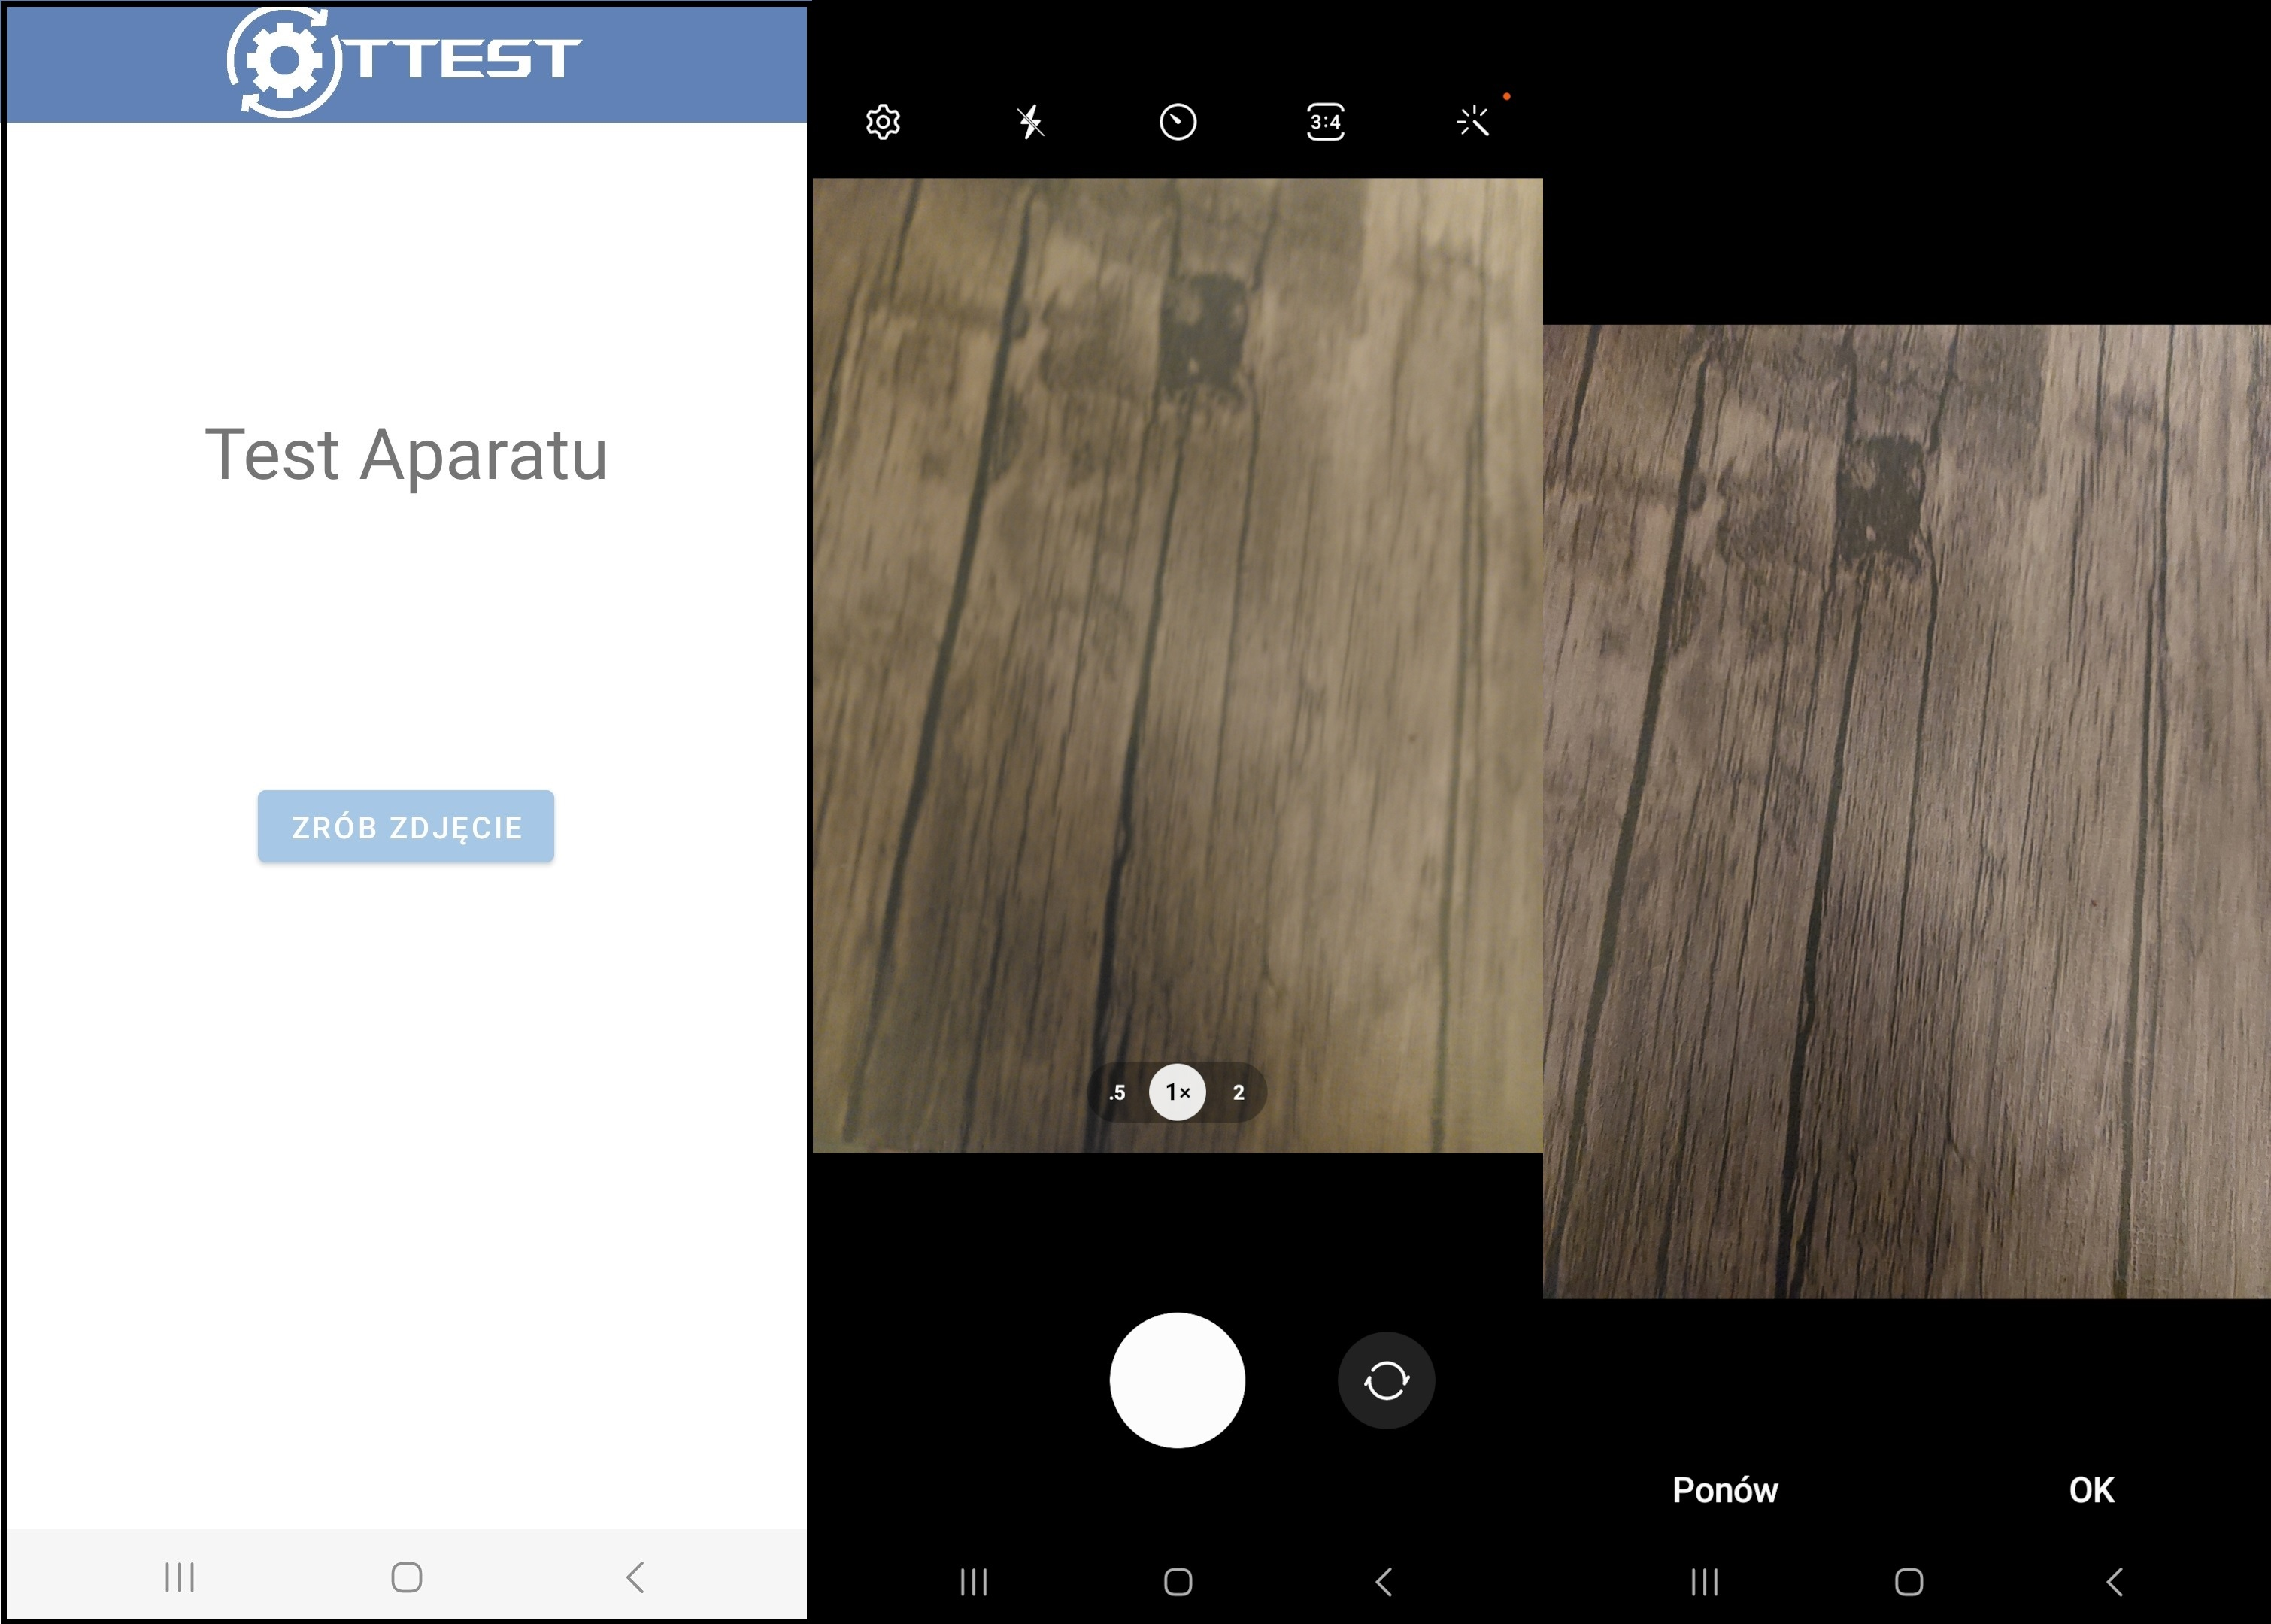
\includegraphics[angle=360, width=0.90\textwidth]{rys/punkt5/aparat.jpg}
		\caption{Przebieg testowania aparatu}
		\label{rys:aparat_5}
	\end{center}
\end{figure} 

\newpage


\subsection{Testowanie menu}

\hspace{0.60cm}Zadania jakie ma spełniać menu przedstawione są w tabeli \ref{tab:tablica_menu}. Jako "X" w kolumnie "Tak" lub "Nie", oznaczamy pomyślny lub niepomyślny przebieg poszczególnych zadań. Całość testu podsumowana jest rzutami ekranu \ref{rys:menu} wykonanymi podczas testowania jako potwierdzenie wykonanego testu.

\begin{tabela}
	{Testowanie menu}	%opis w spisie tabel
	{Testowanie menu}	%opis przy tabeli
	{
		\begin{tabular}{|c|c|c|c|} \hline
			\textbf{lp} & \textbf{Zadania do przetestowania} & \textbf{Tak} & \textbf{Nie} \\ \hline
			1 & Guzik "Latarka" przekierowuje do testu latarki & X & ~ \\ \hline
			2 & Guzik "Tryb ciemny" przekierowuje do testu trybu ciemnego & X & ~ \\ \hline
			3 & Guzik "Zbliżeniowy" przekierowuje do testu czujnika zbliżeniowego & X & ~ \\ \hline
			4 & Guzik "GPS" przekierowuje do testu lokalizacji & X & ~ \\ \hline
			5 & Guzik "Wifi" przekierowuje do testu wifi & X & ~ \\ \hline
			6 & Guzik "Dźwięk" przekierowuje do testu dźwięku & X & ~ \\ \hline
			7 & Guzik "Mikrofon" przekierowuje do testu mikrofonu & X & ~ \\ \hline
			8 & Guzik "Aparat" przekierowuje do testu aparatu & X & ~ \\ \hline
			9 & Guzik "Wyniki" przekierowuje do podsumowania testów & X & ~ \\ \hline
	\end{tabular}	}
	\label{tab:tablica_menu}
\end{tabela}

Rysunek \ref{rys:menu} przedstawia zrzut ekranu potwierdzający pomyślny przebieg testu.

\begin{figure}[!hbt]
	\begin{center}
		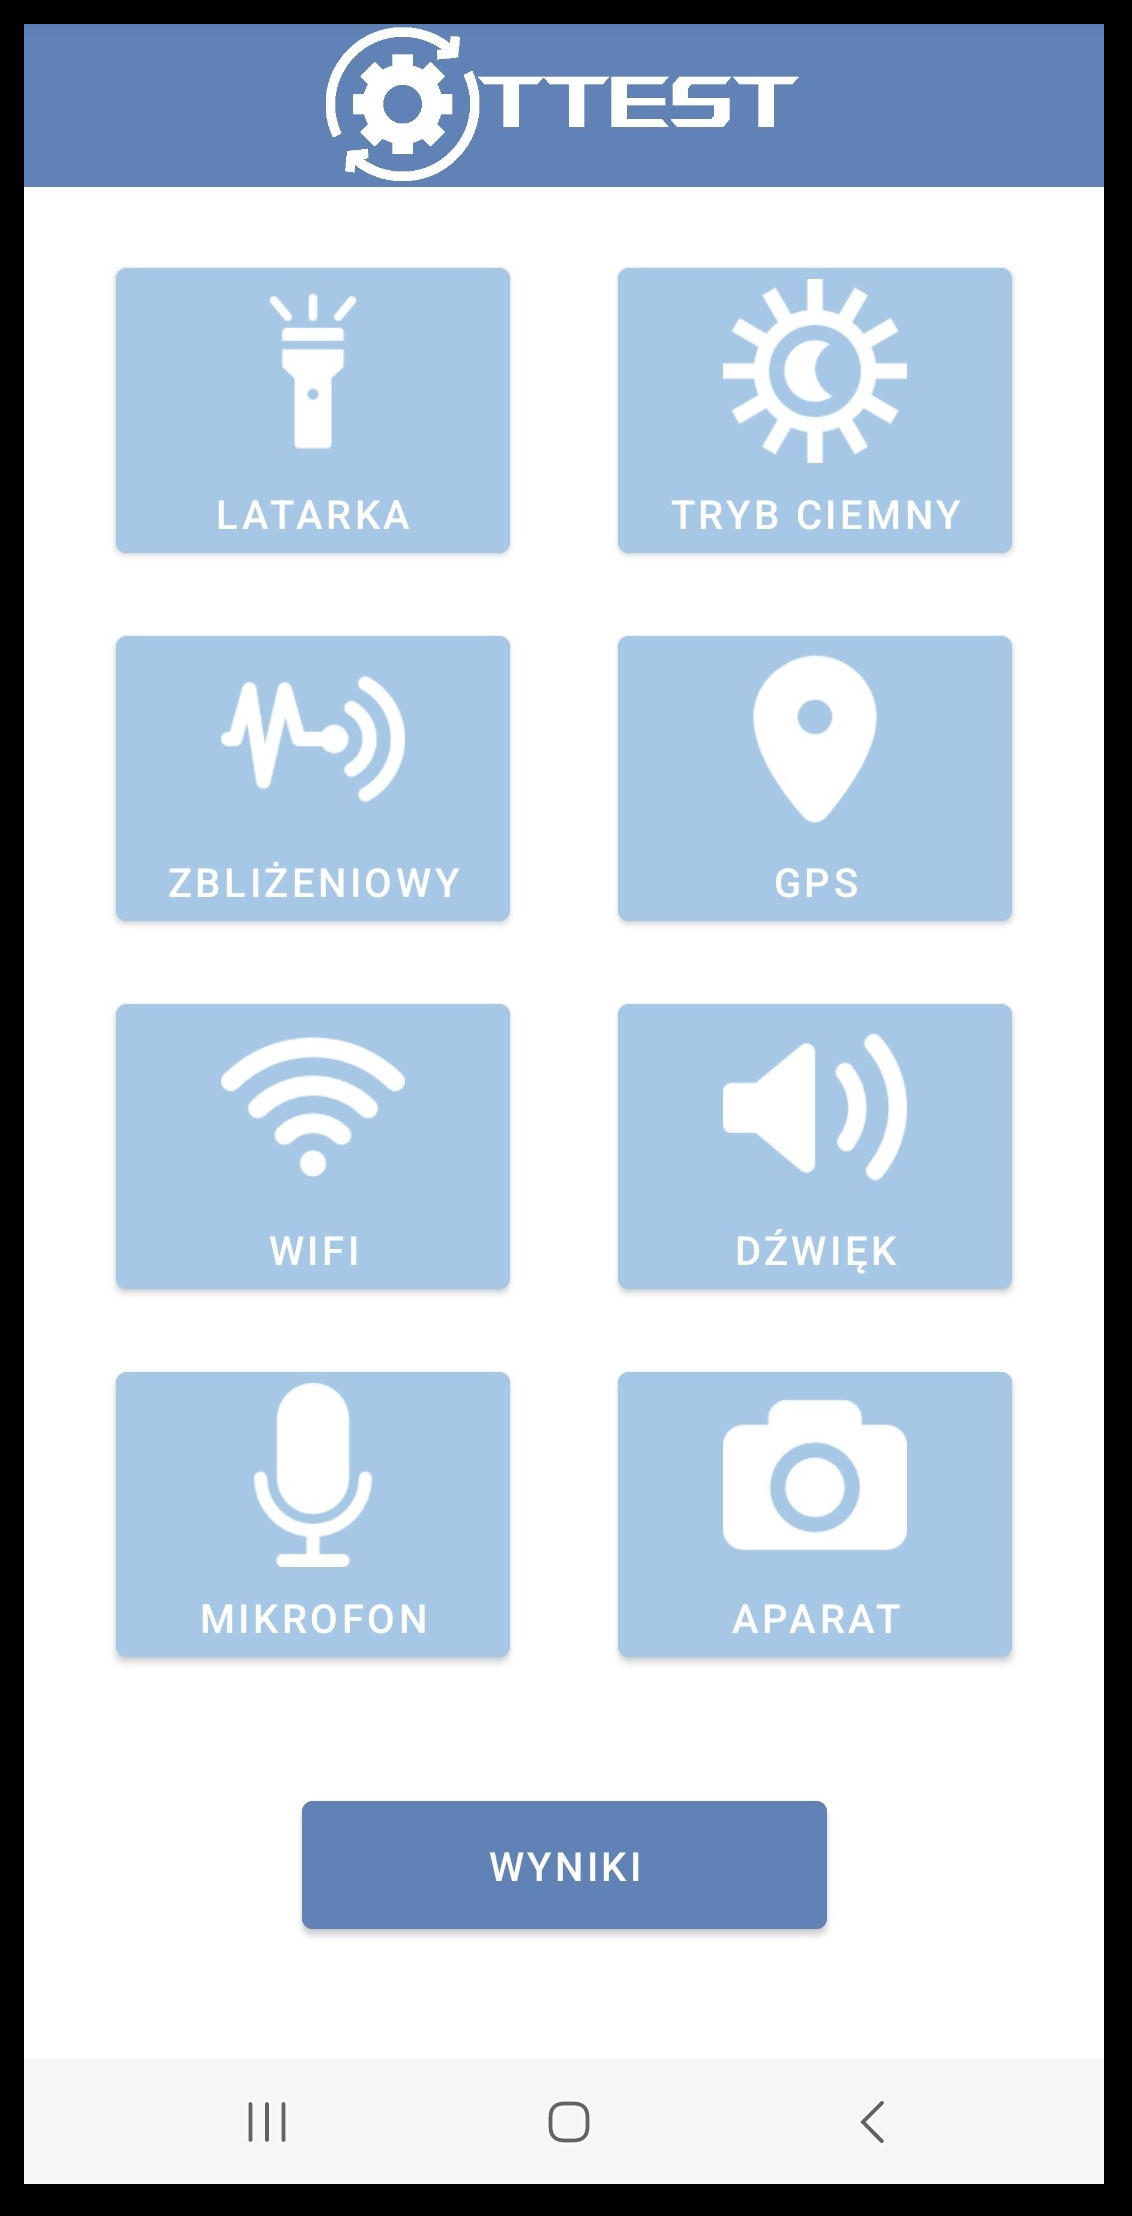
\includegraphics[angle=360, width=0.30\textwidth]{rys/punkt5/menu.png}
		\caption{Przebieg testowania menu}
		\label{rys:menu}
	\end{center}
\end{figure}   

\newpage


\subsection{Testowanie podsumowania}

\hspace{0.60cm}Zadania jakie ma spełniać podsumowanie przedstawione są w tabeli \ref{tab:tablica_wyniki}. Jako "X" w kolumnie "Tak" lub "Nie", oznaczamy pomyślny lub niepomyślny przebieg poszczególnych zadań. Całość testu podsumowana jest rzutami ekranu \ref{rys:wyniki_5} wykonanymi podczas testowania jako potwierdzenie wykonanego testu.

\begin{tabela}
	{Testowanie podsumowania}	%opis w spisie tabel
	{Testowanie podsumowania}	%opis przy tabeli
	{
		\begin{tabular}{|c|c|c|c|} \hline
			\textbf{lp} & \textbf{Zadania do przetestowania} & \textbf{Tak} & \textbf{Nie} \\ \hline
			1 & Wyświetla się informacja o marce i modelu telefonu & X & ~ \\ \hline
			2 & W każdej grupie można wybrać tylko jeden przycisk typu radio & X & ~ \\ \hline
			3 & Po naciśnięciu na guzik pojawia się podsumowanie zaznaczonych opcji & X & ~ \\ \hline
			4 & Pozytywne wyniki testów są wyświetlane na zielono & X & ~ \\ \hline
			5 & Negatywne wyniki testów są wyświetlane na czerwono & X & ~ \\ \hline
	\end{tabular}	}
	\label{tab:tablica_wyniki}
\end{tabela}

Rysunek \ref{rys:wyniki_5} przedstawia zrzuty ekranu potwierdzające pomyślny przebieg testu.

\begin{figure}[!hbt]
	\begin{center}
		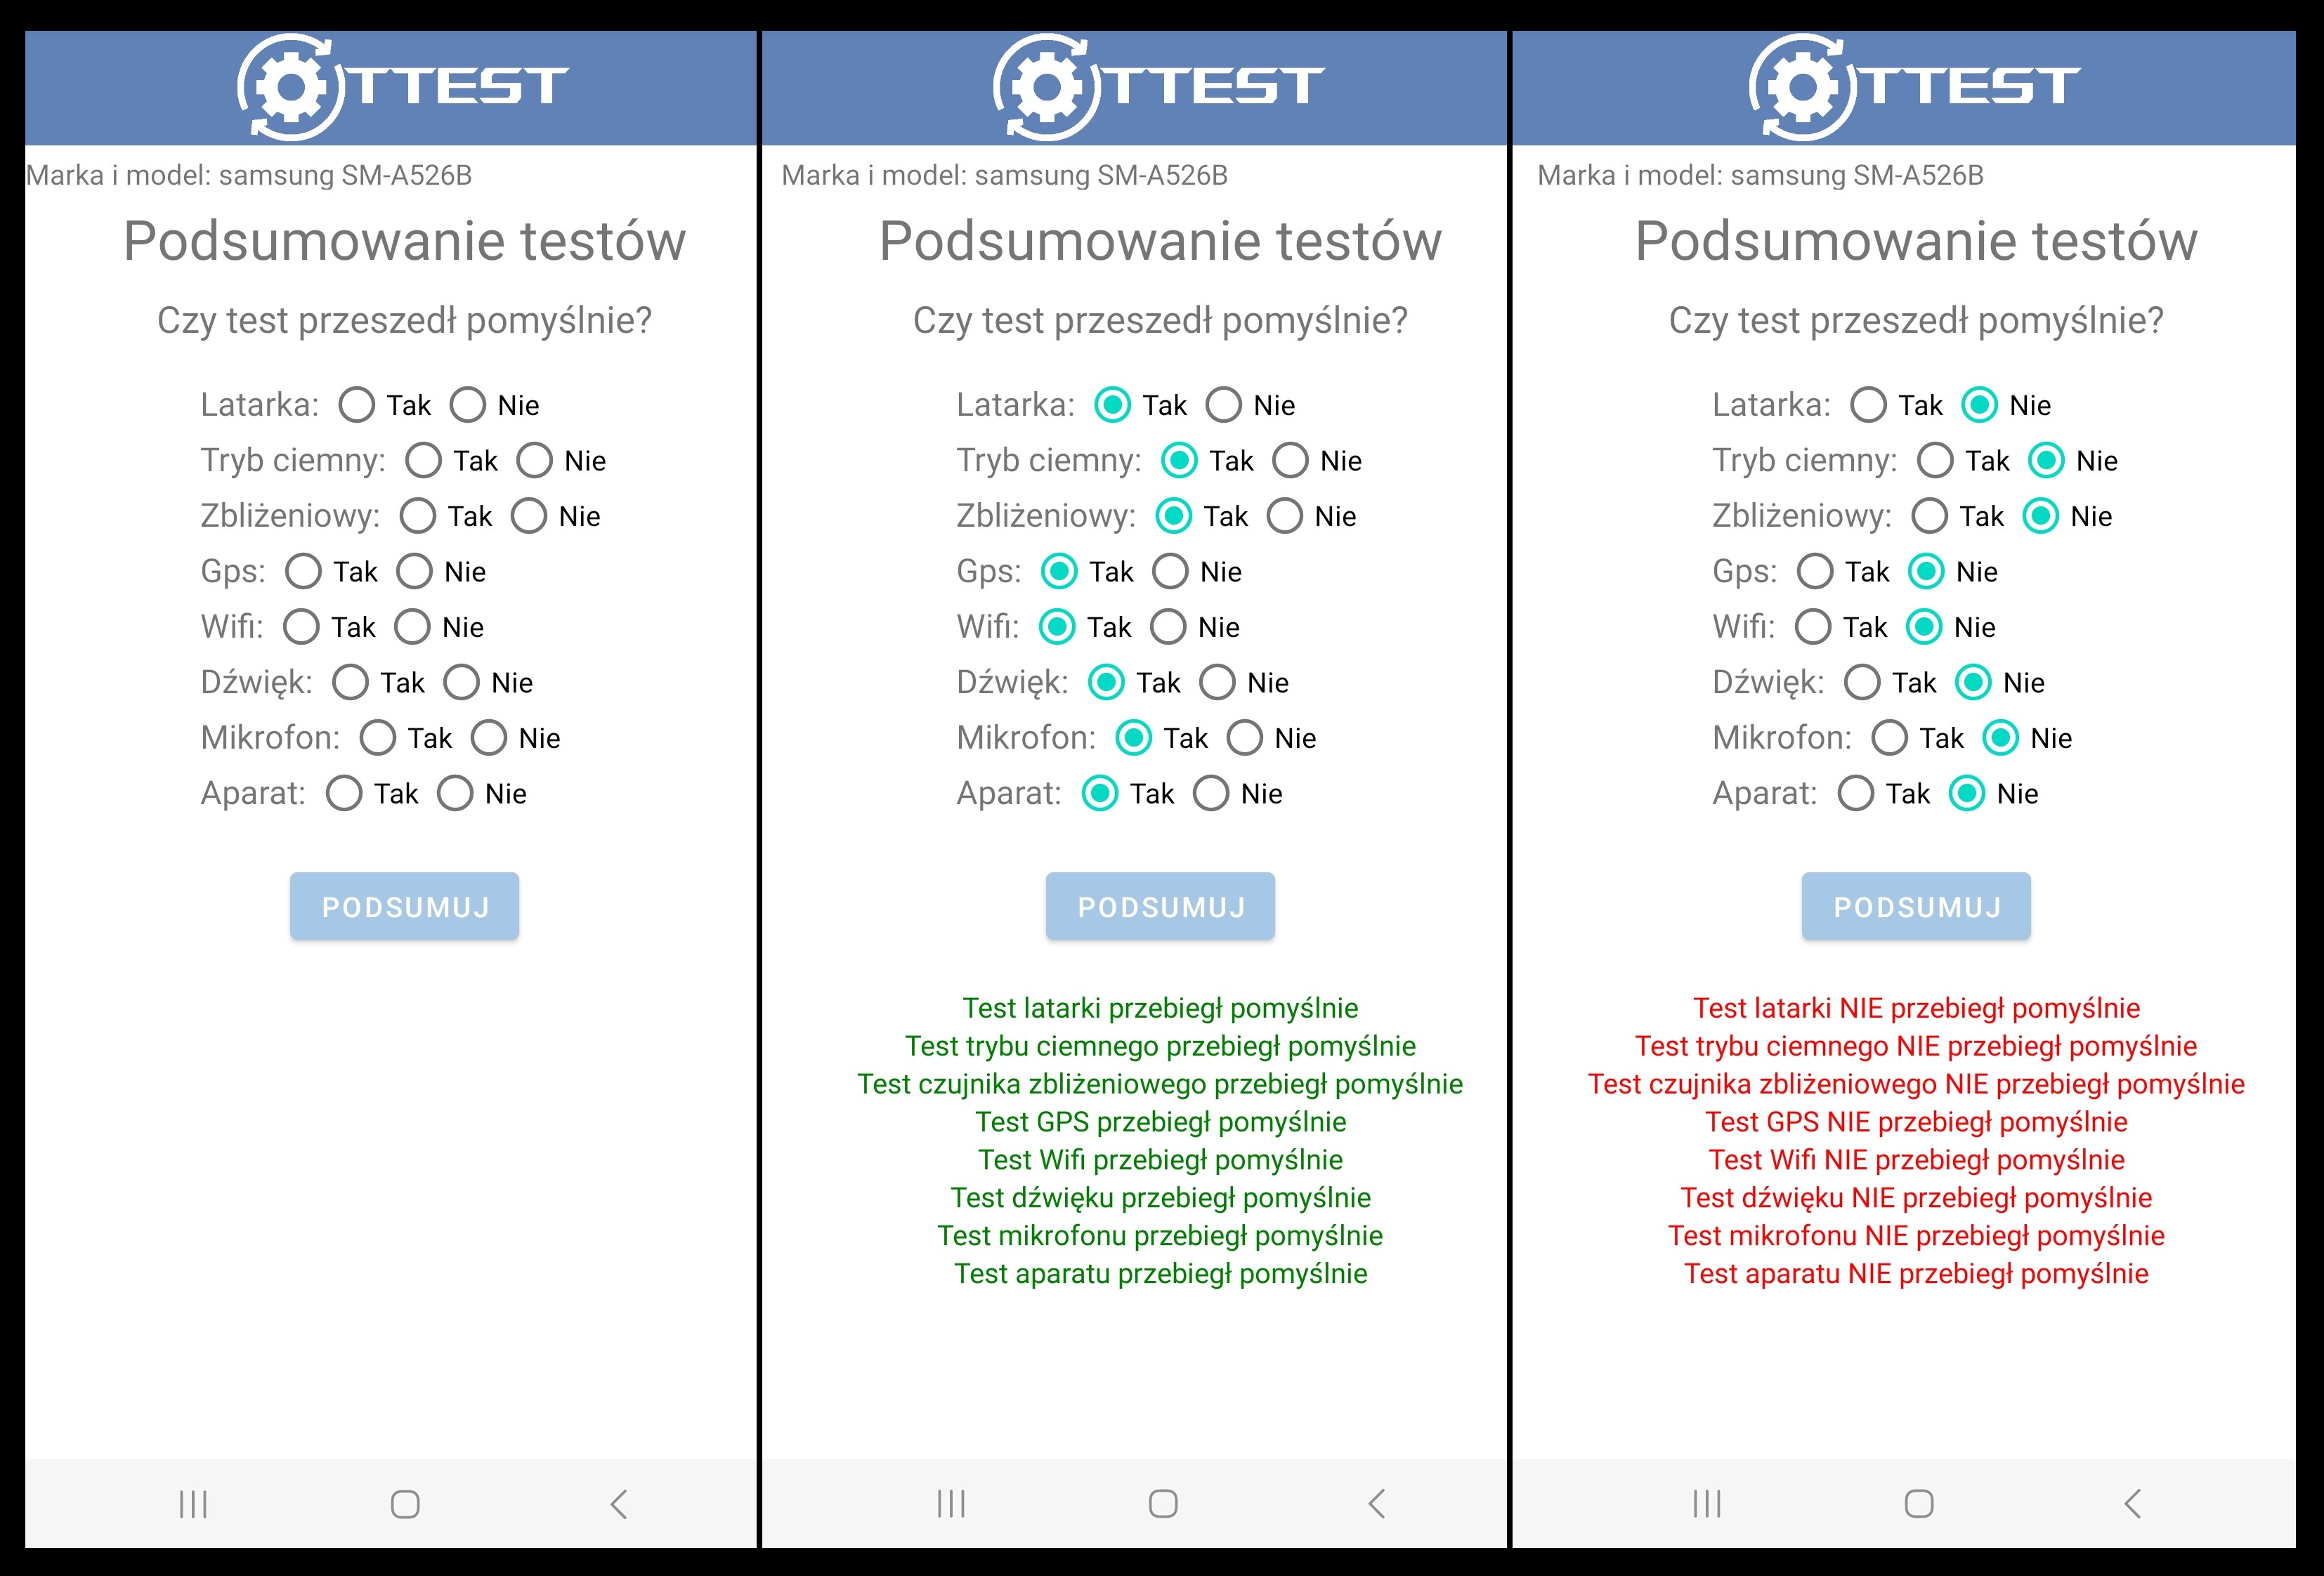
\includegraphics[angle=360, width=0.90\textwidth]{rys/punkt5/wyniki.png}
		\caption{Przebieg testowania podsumowania}
		\label{rys:wyniki_5}
	\end{center}
\end{figure}   

\newpage

